%
% File acl2020.tex
%
%% Based on the style files for ACL 2020, which were
%% Based on the style files for ACL 2018, NAACL 2018/19, which were
%% Based on the style files for ACL-2015, with some improvements
%%  taken from the NAACL-2016 style
%% Based on the style files for ACL-2014, which were, in turn,
%% based on ACL-2013, ACL-2012, ACL-2011, ACL-2010, ACL-IJCNLP-2009,
%% EACL-2009, IJCNLP-2008...
%% Based on the style files for EACL 2006 by 
%%e.agirre@ehu.es or Sergi.Balari@uab.es
%% and that of ACL 08 by Joakim Nivre and Noah Smith

\documentclass[11pt,a4paper]{article}
\usepackage[hyperref]{acl2021}
\usepackage{times}
\usepackage{latexsym}
\usepackage{stfloats}

\renewcommand{\UrlFont}{\ttfamily\small}
\usepackage{amsmath,amsthm,amssymb}

% This is not strictly necessary, and may be commented out,
% but it will improve the layout of the manuscript,
% and will typically save some space.
\usepackage{microtype}
\usepackage{balance}
\usepackage{paralist}
\usepackage{verbatim}
\usepackage[normalem]{ulem}
\usepackage[vlined,ruled,linesnumbered]{algorithm2e}
\usepackage{makecell}
\usepackage{txfonts}
\usepackage{xspace}
\usepackage{booktabs}
\usepackage{graphicx}
\usepackage{xcolor,colortbl}
\usepackage{color,soul}
\usepackage{multirow}

\usepackage[T1]{fontenc}
\usepackage{bbold}
\usepackage{pifont}% http://ctan.org/pkg/pifont


%\aclfinalcopy % Uncomment this line for the final submission
\def\aclpaperid{183} %  Enter the acl Paper ID here

%\setlength\titlebox{5cm}
% You can expand the titlebox if you need extra space
% to show all the authors. Please do not make the titlebox
% smaller than 5cm (the original size); we will check this
% in the camera-ready version and ask you to change it back.
\renewcommand{\ttdefault}{txtt}
\newcommand\BibTeX{B\textsc{ib}\TeX}
%\newcommand*{\emailfont}{\fontfamily{pcr}\selectfont}

\DeclareMathOperator*{\argmax}{arg\,max}
\DeclareMathOperator*{\argmin}{arg\,min}
\DeclareMathOperator*{\dist}{D_f}
\DeclareMathOperator*{\fp}{f_p}
\DeclareMathOperator*{\E}{\mathbf{H}}
\DeclareMathOperator*{\R}{r}
\newcommand{\relation}[1]{\R(#1)}

\setlength{\fboxsep}{0pt}

\newcommand{\colbox}[2]{\colorbox{#1}{#2}}

 
\newcommand{\veryshortarrow}[1][3pt]{\mathrel{%
   \hbox{\rule[\dimexpr\fontdimen22\textfont2-.2pt\relax]{#1}{.4pt}}%
   \mkern-4mu\hbox{\usefont{U}{lasy}{m}{n}\symbol{41}}}}
   
  
\definecolor{caddback}{rgb}{0.90, 0.98, 0.96}
\definecolor{cadd}{rgb}{0, 0.47, 0.34}
\definecolor{cdelback}{rgb}{1, 0.94, 0.92}
\definecolor{cdel}{rgb}{0.83, 0.32, 0.16}
\def \arrow{$\veryshortarrow$}
\newcommand{\add}[1]{\colbox{caddback}{\color{cadd}#1\xspace}} %
\newcommand{\addplus}[1]{{\footnotesize+}\add{#1}}


\newcommand{\remove}[1]{\colbox{cdelback}{{\color{cdel}#1\xspace}}}%
\newcommand{\swap}[2]{\remove{#1}~\arrow~\add{#2}}
\newcommand{\ctrltag}[1]{\texttt{#1}\xspace}
%\renewcommand{\add}[1]{{\color{cadd}#1\xspace}} %





\definecolor{cexample}{rgb}{0.23, 0.30, 0.45}
\newcommand{\exinline}[1]{{\color{cexample}``#1''\xspace}}
\newcommand{\fillin}[1]{{\color{cexample}#1\xspace}}

\newcommand{\fontsmall}{\fontsize{9pt}{11pt}\selectfont}
\newcommand{\fontnormal}{\fontsize{10pt}{12pt}\selectfont}
\fboxrule=0.1pt
\newcommand{\ebox}[1]{%
	%\smallskip
	\vspace{2pt}
	\noindent\fcolorbox{gray}{white}{
		\begin{minipage}{0.95\linewidth}
			\fontsmall
			%\begin{internallinenumbers}
			%\resetlinenumber
			{#1}
			%\end{internallinenumbers}
		\end{minipage}
	}
	\vspace{-2pt}
}

% [(0.166, 'opposing '), (0.099, 'team '), (0.027, 'by '), (0.026, 'quarterback '), (0.024, 'The '), (0.024, 'is '), (0.024, '. '), (0.023, ' '), (0.023, 'about '), (0.023, 'to '), (0.023, 'be '), (0.023, 'tackled '), (0.019, 'the '), (-0.0, ' ')]
%#eef5fa
%#daeaf5
%#c6deef
%#b2d2e9
%#9ec7e4
%#8abbde

\definecolor{ctemplate}{rgb}{0.23, 0.30, 0.45}
%\definecolor{ctemplate}{rgb}{0.23, 0.30, 0.45}
\definecolor{cword}{rgb}{0, 0, 0.7}
\newcommand{\BLANK}{\texttt{BLANK}}

% format
\newcommand{\clabel}[1]{\emph{#1}\xspace}

% constants
\newcommand{\sysname}{\textsc{Polyjuice}\xspace}
\newcommand{\modelurl}{\url{https://huggingface.co/uw-hai/polyjuice}}
\renewcommand{\modelurl}{\texttt{[URL omitted]}}

\newcommand{\mturkurl}{\url{https://tongshuangwu.github.io/perturb-exp-ui/?assignmentId=1&platform=standalone&debug=debug&task=nli}}
\newcommand{\tagstr}{control code\xspace}
\newcommand{\Tagstr}{Control code\xspace}
\newcommand{\tagstrs}{control codes\xspace}
\newcommand{\tagstrshorts}{codes\xspace}
\newcommand{\tagstrshort}{code\xspace}


\newcommand{\cmark}{{\ding{51}}}%
\newcommand{\xmark}{{\ding{55}}}%
\newcommand{\qmark}{{\textbf{\textsf{?}}}}%

\newcommand{\perturbtoken}{\texttt{<|perturb|>}\xspace}%
\newcommand{\stoptoken}{\texttt{[SEP]}\xspace}%



\newcommand{\eg}{\emph{e.g.,}\xspace}%
\newcommand{\ie}{\emph{i.e.,}\xspace}

% tasks
\newcommand{\nli}{\emph{NLI}\xspace}
\newcommand{\sst}{\emph{Sentiment}\xspace}
\newcommand{\qqp}{\emph{QQP}\xspace}

\def \dsst{SST-2\xspace}
\def \dqqp{QQP\xspace}
\def \dnli{SNLI\xspace}


\newcommand{\xp}{\hat{x}}
\newcommand{\yp}{\hat{y}}
\newcommand{\xset}{\mathbf{X}}
\newcommand{\tofix}[1]{{\color{red}#1}\xspace}


% annotations
\newcommand{\ensuretext}[1]{#1}
\newcommand{\marker}[2]{\ensuremath{^{\textsc{#1}}_{\textsc{#2}}}}
\newcommand{\arkcomment}[3]{\ensuretext{\textcolor{#3}{[#1 #2]}}}
%\renewcommand{\arkcomment}[3]{}  % uncomment for submission
\newcommand{\hao}[1]{\arkcomment{\marker{H}{P}}{#1}{purple}}
\newcommand{\wts}[1]{\arkcomment{\marker{S}{W}}{#1}{orange}}
\newcommand{\victor}[1]{\arkcomment{\marker{V}{Z}}{#1}{blue}}
\newcommand{\dq}[1]{\arkcomment{\marker{D}{Q}}{#1}{cyan}}
\newcommand{\dan}[1]{\arkcomment{\marker{D}{W}}{#1}{red}}

% teal, cyan
%\title{\sysname: General-purpose Counterfactual Generation}
\title{\sysname: Generating Counterfactuals \\for Explaining, Evaluating, and Improving Models}


\author{
\makecell{
Tongshuang Wu$^{1}$ ~~~~~~~ 
Marco Tulio Ribeiro$^{2}$ ~~~~~~~ 
Jeffrey Heer$^{1}$ ~~~~~ 
Daniel S. Weld$^{1,3}$}  \\ 
$^{1}$University of Washington\hspace{5mm}
$^{2}$Microsoft Research\hspace{5mm} 
$^{3}$Allen Institute for Artificial Intelligence\hspace{5mm}\\
\hspace{-5mm}
\href{mailto:wtshuang@cs.uw.edu}{\texttt {wtshuang@cs.uw.edu}}
\hspace{5mm}
\href{mailto:marcotcr@microsoft.com}{\texttt {marcotcr@gmail.com}}
\hspace{10mm}
\href{mailto:dan@cs.washington.edu}{\texttt {\{jheer,weld\}@cs.uw.edu}}
}


\date{}

\begin{document}
\maketitle
\begin{abstract}


While counterfactual examples
%(or perturbations) \dq{} 
are useful for analysis and training of NLP models, current generation methods either rely on manual labor to create very few counterfactuals, or 
%only instantiate a small set of automatic perturbations such as paraphrases or word substitutions.
only instantiate limited types of perturbations such as paraphrases or word substitutions. %, lacking variety.
We present \sysname, a general-purpose counterfactual generator that allows for control over perturbation types and locations, trained by finetuning GPT-2 on multiple datasets of paired sentences. 
We show that \sysname produces diverse sets of realistic counterfactuals, which in turn are useful in various distinct applications: improving training and evaluation on three different tasks (with up to 75\% less annotation effort than manual generation), augmenting state-of-the-art explanation techniques, and supporting systematic counterfactual error analysis that reveals behaviors easily missed by human experts.

% Counterfactual examples are useful for various applications, but current methods for generating them either rely on crowdsourcing, or only instantiate a small set of possible perturbations-of-interest (\eg changing the groundtruth label through a single antonym substitution.)
% We propose \sysname, a general purpose counterfactual generator, by finetuning GPT-2 on multiple datasets with paired sentences. 
% \sysname allows control over the type and location of perturbations, and therefore more comprehensively cover desired counterfactuals.
% We show that \sysname produces a diverse set of fluent counterfactuals, and that simple selection mechanisms make it useful for training and evaluation (up to 75\% less annotation effort compared to manual creation), augments state-of-the-art explanation techniques, and supports counterfactual error analysis by revealing erroneous model behaviors that are easily missed by human analysts.


%Counterfactual examples have been shown to be useful for many applications, including calibrating, evaluating, and explaining model decision boundaries. 
%However, previous methods for generating such counterfactuals have been tightly tailored to a specific application, used a limited range of linguistic patterns, or are hard to scale. 
%We propose to disentangle counterfactual generation from its use cases, \ie gather general-purpose counterfactuals first, and then select them for specific applications. 
%We frame the automated counterfactual generation as text generation, and finetune GPT-2 into a generator, \sysname, which produces fluent and diverse counterfactuals. 
%Our method also allows control over where perturbations happen and what they do. 
%We show \sysname supports multiple use cases: 
%When creating datasets for model training and evaluation, \sysname helps to save up to 75\% annotation efforts over manual creation.
%When used to produce explanations and for error analysis, \sysname reveals erroneous model behaviors that are easily missed by human analysts.



%
%Existing methods generate counterfactual examples for specific applications, even though most of the examples can be broadly used for calibrating, evaluating, and explaining model decision boundaries. 
%Constrained by their use cases, the methods each have a limited linguistic pattern coverage or are hard to scale. 
%We propose to disentangle the generation from the use cases, \ie, gather general-purpose counterfactuals first, and then select them for specific applications. 
%We frame the automated counterfactual generation as text generation, and finetune GPT-2 into a generator, \sysname, which produces fluent and diverse counterfactuals. 
%It also allows control over where perturbations happen and what they do. With effective selections, we show \sysname supports multiple use cases: by generating diverse counterfactuals for humans to label, \sysname helps produce high-quality datasets for model training and evaluation, with at least 40\% less human effort. 
%As counterfactual explanations, \sysname helps reveal erroneous model behaviors on top of popular feature attribution methods. 
\end{abstract}

\section{Introduction}
\label{sec:intro}



Counterfactual reasoning --- mentally simulating what \emph{would have happened} if conditions were different --- is a common tool for making causality assessments~\cite{kahneman}, which in turn are crucial for model training, evaluation, and explanation~\cite{miller}. 
For example, in Figure~\ref{fig:teaser}, \exinline{It is great for kids} is perturbed into multiple variations, each providing unique insights by simulating what would have happened if the sentence was different.

Applications of counterfactual reasoning to NLP generally specify the relationship $x \veryshortarrow \xp$, and then create $\xp$ according to the relationship.
As a result, prior work has tailored counterfactual generators for every application, which induces different limitations.
%For example, a minimal edit of a sentence $x$ that results in a different label is useful for model training and evaluation.
%Such counterfactuals are usually produced manually by human annotators ~\cite{gardner2020contrast} or by human-written perturbation functions~\cite{wu2019errudite}, making them costly to generate (\eg 4-5 minutes per counterfactual \cite{kaushik2019learning}) and liable to systematic omissions (\eg human annotators may miss \swap{kids}{no one} in Figure \ref{fig:teaser}B). %Further, relying on human creativity may cause important but non-obvious patterns to be missed, \eg humans may cover \swap{great}{not great}, but miss \swap{kids}{no one} in Figure~\ref{fig:teaser}B.
%Though it is cheaper to automate the process with parsing templates~\cite{li2020linguistically}, the templates usually have limited coverage on either the patterns-to-perturb, or the applicable data points.
%In contrast, adversarial examples specify a very different counterfactual relationship: $x$ and $\xp$ must have different model predictions \emph{despite} being semantically equivalent, such that automated methods often rely on paraphrasing models~\cite{iyyer2018adversarial, ribeiro2018semantically}.
For example, to support model training and evaluation, human annotators collect counterfactuals that change the groundtruth labels by manually rewriting instances~\cite{gardner2020contrast} or defining perturbation functions~\cite{wu2019errudite}.
The manual rewrites are costly (\eg 4-5 minutes per counterfactual \cite{kaushik2019learning}) and liable to systematic omissions (\eg human annotators may miss \swap{kids}{no one} in Figure \ref{fig:teaser}B).
The focus on label-flipping relationships also largely ignores the benefit from label-preserving ones on model robustness.
In contrast, adversarial examples specify a different relationship: $x$ and $\xp$ must have the same groundtruth but different model predictions, driving the generator to prioritize straightforward paraphrasing~\cite{iyyer2018adversarial, ribeiro2018semantically}, over alternatives that change the semantic meaning (\eg negations in named entity recognition).
% or synonym replacement

\begin{figure}[t]
\centering
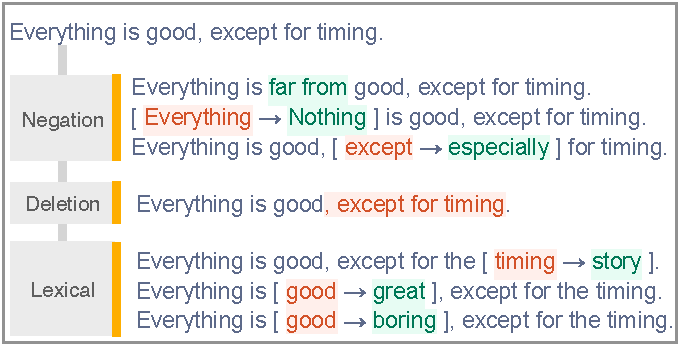
\includegraphics[trim={0 18cm 30.5cm 0cm},clip, width=1\columnwidth]{figures/teaser.pdf}
\vspace{-15pt}
\caption{
Overview: (A) given a sentiment analysis instance $x$, \sysname generates (B) a large set of counterfactuals $\xp$, which are then (C) selected for downstream use.
For example, in (D) we select counterfactual explanations that complement the feature attributions: though both ``great'' and ``kids'' are deemed important, perturbing them may not affect the prediction $f(x)=f(\xp)=\text{\emph{positive}}$, revealing model errors.\footnotemark
}
\vspace{-10pt}
\label{fig:teaser}
\end{figure} 
\footnotetext{We open source both the \sysname model and the selection strategies at \modelurl.}


%However, as Figure \ref{fig:teaser} illustrates, counterfactual generation does not \emph{have} to be task-specific, as various applications share similar requirements on $x\veryshortarrow\xp$ (\eg a preference for small changes).
%In fact, a general-purpose pool of diverse counterfactuals may be preferable when the relationship is not precisely defined in advance, as is the case for counterfactual training, evaluation, or explanations.
% In fact, a common pool of counterfactuals may support each application more comprehensively.
% For example, without the preset constrain on semantic equivalence, we can collect adversarials through negation (for tasks insensitive to negation, \eg named entity recognition.)
%For example, some forms  in training and evaluation data collection can 
%The exhaustive search of automated methods can cover the training and evaluation more comprehensively, and non-paraphrasing changes like \emph{add negation} are valuable adversarials for tasks like named entity recognition. 
%\hao{might be good to clarify that these two are not mutually-exclusive: adversarial examples should sometimes be close to the original}
% 
However, counterfactual generation does not \emph{have} to be task-specific.
The same set of counterfactuals in Figure~\ref{fig:teaser} can support a variety of applications.
Moreover, for cases like counterfactual explanation (Figure~\ref{fig:teaser}D) and analysis, a general-purpose pool of counterfactuals is preferable, as the relationship-of-interest can be more open-ended and user oriented.
In this work, we formalize the task of \emph{counterfactual generation}, which disentangles generation from the application of counterfactuals (\S\ref{sec:general_purpose}).
Given an input $x$, our generator produces a set of counterfactuals $\hat{\xset} = \{\xp_1, \xp_2, ...\}$ with \emph{application-agnostic} relationships $x \veryshortarrow \xp_i$ (Figure~\ref{fig:teaser}B).
Afterwards, we use \emph{application-specific} selection methods to find subsets of $\xp$ that are most effective for a use case (Figure~\ref{fig:teaser}C).
We frame the generation step as conditional text generation, and finetune GPT-2~\cite{radford2019language} into a generator called \emph{\sysname} using $(x, \xp)$ pairs. 
We also allow for targeted counterfactuals, by specifying where the perturbation occurs~\cite{donahue2020enabling} and using \tagstrs like \ctrltag{negation} or \ctrltag{delete} (Figure~\ref{fig:teaser}B).
Intrinsic evaluations show that \sysname generate $\xp$ that are \emph{fluent}, \emph{diverse}, \emph{controllable}, and \emph{close to $x$}.

%--- the control is \emph{the backbone of} various downstream applications.

%We propose simple yet effective selection strategies, 
With simple selection heuristics, we show that a single \sysname model can significantly aid humans in diverse downstream applications.\footnote{We demonstrate \sysname in semi-automatic settings, but as discussed in \S\ref{subsec:nlg}, it can also work automatically.} 
For \emph{counterfactual training and evaluation} (\S\ref{sec:app_label}), humans label \sysname counterfactuals rather than creating them from scratch, resulting in training data that significantly improves model generalization, as well as high-quality contrast sets~\cite{gardner2020contrast}, with 40--75\% less annotation effort ~\cite{kaushik2019learning}. 
In another application, \sysname produces \emph{counterfactual explanations} (\S\ref{sec:app_explain}) that bring significant insights that extend beyond state-of-the-art explanation techniques. 
Finally, \sysname supports counterfactual \emph{error analysis} (\S\ref{sec:app_err_analysis}) by allowing users to explore related counterfactuals (\eg the model responds differently to different negation forms in Figure \ref{fig:teaser}B) and to aggregate individual counterfactuals into patterns in order to systematically understand model behavior.

%First, 
% By lifting the burden of manual rewrite, \sysname \emph{facilitates effective counterfactual training and evaluation}.
% With humans only \emph{labeling} counterfactuals, we produce training data that improves model generalization, as well as high-quality contrast sets~\cite{gardner2020contrast} with 40\%--75\% less annotation effort compared to creating them from scratch~\cite{kaushik2019learning}. 
%We similarly produce training data that improves model generalization in three classification tasks. %, when compared to adding the same amount of non-counterfactual data.

% (2) 
% %Second, 
% By generating nontrivial counterfactuals beyond paraphrasing and human intuitions, \sysname helps \emph{produce counterfactual explanations} that highlight model errors obscure to humans. 
% In a user study, experts only did slightly better than random (accuracy: $55 \pm 6\%$) at predicting what a model would do on \sysname counterfactuals, even after inspecting the model on their own.
% (3) 
% %Third, 
% By rewriting each instance in multiple ways, \sysname \emph{supports more systematic error analysis}.
% Case studies demonstrate that \sysname counterfactuals help contrast model behaviors on related perturbations (\eg the model in Figure~\ref{fig:teaser} responds differently to the two negation forms.)

% We opensource both the \sysname model and the selection strategies at \modelurl.


\begin{comment}
In summary, we:
\begin{compactenum}
\item  Formalize the general-purpose counterfactual generation task. 
By \emph{separating the generation from the use cases}, we generate fluent and diverse counterfactuals that bypass application-specific constraints.
%. \hao{maybe emphasize the benefits of this}
\item Finetune a generator called \sysname, by collecting paired sentences and enhancing controls with infilling structures and \tagstrs --- the control is \emph{the backbone of} various downstream applications.
%\sysname generates plausible and diverse counterfactuals, with control over where perturbations happen and what they do.
The model is at \modelurl.
%, and we plan to opensource the selection strategies.
\item Apply \sysname to \emph{model training, evaluation, and explanation}, using various selection methods (which we will opensource).
\sysname helps collect high-quality training and evaluation data with 40\% less annotation effort, and find model bugs that on top of feature attribution explanations and counterfactual analysis.
\end{compactenum}
\wts{Maybe can delete if we run out of space.}
\end{comment}

% we observe that \sysname explanations can complement popular feature attribution methods and highlight their blind spots.
% After viewing SHAP weights~\cite{NIPS2017_7062} and interacting with the model, experts still could not predict model behaviors on counterfactuals selected for explanations, and missed 5\% and 25\% more cases than the human-generated or random baselines.

\section{Task Formalization \& Modeling}

\begin{comment}
* Define the task
- Some math
- Several different application domains
    - augmentation
    - adversarial attack
    - extend data
    - counterfactual explanation
- Importance of where to change and how to change

* How to train
- Compute control tags
- Special tokens

* Use existing datasets
- Why each dataset 
- Data distribution [maybe appendix]

* Training hyperparameters

* Evaluations
- Filtering
- Diversity
\end{comment}


@article{gardner2020contrast,
  title={Evaluating models' local decision boundaries via contrast sets},
  author={Gardner, Matt and Artzi, Yoav and Basmova, Victoria and Berant, Jonathan and Bogin, Ben and Chen, Sihao and Dasigi, Pradeep and Dua, Dheeru and Elazar, Yanai and Gottumukkala, Ananth and others},
  journal={Findings of EMNLP},
  year={2020}
}

@article{kaushik2019learning,
  title={Learning the difference that makes a difference with counterfactually-augmented data},
  author={Kaushik, Divyansh and Hovy, Eduard and Lipton, Zachary C},
  journal={arXiv preprint arXiv:1909.12434},
  year={2019}
}

@article{kaushik2020explaining,
  title={Explaining The Efficacy of Counterfactually-Augmented Data},
  author={Kaushik, Divyansh and Setlur, Amrith and Hovy, Eduard and Lipton, Zachary C},
  journal={arXiv preprint arXiv:2010.02114},
  year={2020}
}

@article{teney2020learning,
  title={Learning what makes a difference from counterfactual examples and gradient supervision},
  author={Teney, Damien and Abbasnedjad, Ehsan and Hengel, Anton van den},
  journal={arXiv preprint arXiv:2004.09034},
  year={2020}
}


@article{sakaguchi2019winogrande,
  title={Winogrande: An adversarial winograd schema challenge at scale},
  author={Sakaguchi, Keisuke and Bras, Ronan Le and Bhagavatula, Chandra and Choi, Yejin},
  journal={arXiv preprint arXiv:1907.10641},
  year={2019}
}

@article{zhang2019paws,
  title={PAWS: Paraphrase adversaries from word scrambling},
  author={Zhang, Yuan and Baldridge, Jason and He, Luheng},
  journal={arXiv preprint arXiv:1904.01130},
  year={2019}
}

\newcommand{\tagdefine}[1]{\emph{{\color{darkgray}#1} }}
\renewcommand{\arraystretch}{1.1}
\begin{table*}
\small
\centering
\begin{tabular}{p{0.11\linewidth} p{0.6\linewidth}  p{0.2\linewidth}}
\toprule
\textbf{Code} & \textbf{Definitions and Examples} & \textbf{Datasets} \\ 
\midrule
\ctrltag{Negation}
    & You'd \swap{figure that out}{never know} by watching it though.
    & \cite{kaushik2019learning, gardner2020contrast}
\\ \midrule
\ctrltag{Quantifier}
    & Where can buy Jordan \swap{5}{6} shoes?
    & \cite{gardner2020contrast}
\\ \midrule
\ctrltag{Lexical}
    & \tagdefine{Changing just one word or noun chunks without breaking the POS tags.} \newline
      He found them \swap{exciting}{dull}.
    & \cite{sakaguchi2019winogrande}
\\ \midrule
\ctrltag{Re-semantic}
    & \tagdefine{To replace short phrases or clauses without affecting the parsing tree.}\newline
      How do you \swap{access Snapchat}{brand yourself} online?
    & \cite{zhang2019paws}
\\ \midrule
\ctrltag{Insert}
    & \tagdefine{To add constraints without affecting the parsing structure of other parts.} \newline
      I liked a \add{Bangali} boy.
    & \cite{zhang2019paws, gardner2020contrast}
\\ \midrule
\ctrltag{Delete}
    & \tagdefine{To remove constraints without affecting the parsing structure of other parts.} \newline
    The lawyers paid \remove{the tourists}.
    & \cite{zhang2019paws, gardner2020contrast}
\\
\ctrltag{Delete}
    & \tagdefine{To remove constraints without affecting the parsing structure of other parts.} \newline
    The lawyers paid \remove{the tourists}.
    & \cite{zhang2019paws, gardner2020contrast}
\\
\bottomrule
\end{tabular}
\caption{Examples of extracted top (topics) using Empath~\cite{Fast2016EmpathUT} and original messages. Empath could correctly extract most topics ({\em e.g.}, \emph{``competing''}) from greeting card messages, but might also be misled by the frequent occurrence of some keywords and extracts unwanted topics ({\em e.g.}, \emph{``crime''}).}
% We want to extract good topics like ``competing'' that has diverse keywords, and crime is an example of what we filtered. \sherry{Just use one color to highlight related words, no need to distinguish between them; And, add captions saying competing is a good topic and crime is a sample of what we filtered and rectified.}}
\label{table:examples}
\end{table*}


In response to the objectives, we form the perturbation as a text generation task.
Given a paired sentence $x$ and $x'$, We form the training prompts as 


and finetune GPT-2 model

To control \emph{where to change}

\newcommand{\maug}{\texttt{aug}\xspace}
\newcommand{\mcomp}{\texttt{comp}\xspace}

\definecolor{ccon}{HTML}{fee9d4}
\definecolor{cood}{HTML}{d8f0d3}
\definecolor{cid}{HTML}{dae8f5}

\newcommand{\TableAugSST}{
\begin{table*}
\small
\centering
\setlength{\tabcolsep}{4pt}
\begin{tabular}{rrlllllllll}
\toprule
    $n$ &     $m$ &    model & 
    \cellcolor{cid}SST-2 & 
    \cellcolor{cood}Senti140 & 
    \cellcolor{cood}SemEval & 
    \cellcolor{cood}Amzbook & 
    \cellcolor{cood}Yelp & 
    \cellcolor{cood}IMDB & 
    \cellcolor{ccon}IMDB-Cont. & 
    \cellcolor{ccon}IMDB-CDA \\
\midrule
 4,000 &  2,000 &     \mcomp &  $92.9\pm 0.2$ &  $88.9\pm 0.3$ &  $84.8\pm 0.5$ &  $85.1\pm 0.4$ &  $90.0\pm 0.3$ &  $90.8\pm 0.5$ &  $92.2\pm 0.6$ &  $86.5\pm 0.2$ \\
 4,000 &  2,000 &  \maug	 &  $92.7\pm 0.2$ &  $\mathbf{90.7\pm 0.4}$ &  $\mathbf{86.4\pm 0.1}$ &  $85.6\pm 0.8$ &  $90.1\pm 0.0$ &  $90.6\pm 0.3$ &  $\mathbf{94.0\pm 0.3}$ &  $\mathbf{89.7\pm 0.5}$ \\
 % imdb_contrast_test: 91.1 (9.4) / 92.8 (0.4)
 % imdb_contrast_test: 87.4 (0.0) / 89.6 (0.5)
 % imdb_iclr_test 93.0 (0.3) / 93.9 (0.4)
 % imdb_iclr_dev 92.0 (0.2) / 92.7 (0.2)
\bottomrule
\end{tabular}
\vspace{-5pt}
\caption{\sst model performances. 
\maug maintains the \colbox{cid}{in-domain} and \colbox{cood}{out-of-domain} accuracies on reviews (SST-2, Amzbook, Yelp, IMDb Movie Review~\cite{ni2019justifying, asghar2016yelp, maas2011learning}), but improves on Twitter data (Senti140 and SemEval 2017~\cite{go2009twitter, rosenthal2017semeval}), likely because their distribution are less similar to SST-2 than the reviews.
The model also improves on the \colbox{ccon}{contrast sets} (IMDb-Contrast and IMDb-CAD~\cite{gardner2020contrast, kaushik2019learning}).
%on \colbox{cid}{in domain}, \colbox{cood}{out of domain}, and \colbox{ccon}{contrast sets}. \maug performs better than \mcomp on twitter datasets (Senti140~\cite{go2009twitter}, SemEval 2017~\cite{rosenthal2017semeval}) and contrast sets IMDb-Contrast~\cite{gardner2020contrast} and IMDb-CAD~\cite{kaushik2019learning}, while maintaining the ones on reviews (SST-2, Amzbook~\cite{ni2019justifying}, Yelp~\cite{asghar2016yelp}, IMDb Movie Review~\cite{maas2011learning}).
}
\vspace{-5pt}
\label{table:aug_sst}
\end{table*}}

%%%%%%%%%%%%%%%%%%%%%%%%%%%%%%%%%%%%%%%%%%%%%%%
\newcommand{\TableAugNLI}{
\begin{table*}
\small
\centering
\setlength{\tabcolsep}{4pt}
\begin{tabular}{rrlllllllll}
\toprule
     $n$ &     $m$ &    model & \cellcolor{cid}SNLI & \cellcolor{cood}MNLI-m & \cellcolor{cood}MNLI-mm & \cellcolor{ccon}SNLI-CDA & \cellcolor{ccon}break & \cellcolor{ccon}DNC & \cellcolor{ccon}stress & \cellcolor{ccon}diagnostic \\
\midrule
 20,000 &  1,574 &     \mcomp 	&  $85.7\pm 0.4$&  $86.1\pm 0.2$&  $86.6\pm 0.2$&  $72.8\pm 0.3$&  $86.4\pm 1.5$&  $54.5\pm 0.6$&  $65.1\pm 0.6$&  $56.0\pm 0.8$\\
% 20,000 &  1,574 &  \texttt{aug} &  $85.7\pm 0.4$ &  $86.1\pm 0.1$ &  $86.2\pm 0.1$ &  $73.4\pm 0.5$ &  $87.2\pm 0.6$ &  $54.7\pm 0.3$ &  $64.6\pm 0.6$ &  $56.9\pm 0.8$ \\
 20,000 &  1,574 &  \maug	&  $85.3\pm 0.3$&  $86.0\pm 0.1$&  $86.4\pm 0.0$&  $\mathbf{73.6\pm 0.2}$&  $\mathbf{89.1\pm 1.2}$&  $\mathbf{57.7\pm 0.3}$&  $65.1\pm 0.2$&  $\mathbf{57.5\pm 0.5}$\\
 %10000 &  1574 &     comp &  $85.3\pm 0.5$&  $85.2\pm 0.2$&  $85.4\pm 0.3$&  $72.4\pm 0.1$&  $86.1\pm 1.8$&  $54.2\pm 1.8$&  $64.0\pm 0.4$&  $56.0\pm 0.3$\\
 %10000 &  1574 &  aug\_gpt &  $85.3\pm 0.3$&  $85.0\pm 0.2$&  $85.1\pm 0.1$&  $73.4\pm 0.5$&  $90.5\pm 1.1$&  $56.5\pm 1.2$&  $64.6\pm 0.5$&  $57.0\pm 0.4$\\
\bottomrule
\end{tabular}
\vspace{-5pt}
\caption{\nli model performances. 
\maug performs better than \mcomp on DNC~\cite{kim2019probing}, which is the target of the augmentation. It also improves on other \colbox{ccon}{contrast/challenge sets}~\cite{naik2018stress, glockner-etal-2018-breaking, wang2018glue},  while maintaining the \colbox{cid}{in domain}, \colbox{cood}{out of domain}~\cite{williams-etal-2018-broad} accuracies.}
\vspace{-5pt}
\label{table:aug_nli}
\end{table*}
}

%%%%%%%%%%%%%%%%%%%%%%%%%%%%%%%%%%%%%%%%%%%%%%%
\newcommand{\TableAugQQP}{
\begin{table}
\small
\centering
\setlength{\tabcolsep}{4pt}
\begin{tabular}{p{0.4\textwidth} r}
\toprule
TESTNAME &   $\Delta$ fail\%  \\
\midrule
 Order does not matter for symmetric relations &  -18.4\% \\
 Order does not matter for comparison &  -26.5\% \\
 Order does matter for asymmetric relations &  -14.5\% \\
%\midrule
% Is it \{ok, bad,..\} to \{smoke, do,..\} \{\emph{before $\not\eq$ after}\} &  -52.5\% \\
% %What was person's life \{\emph{before $\not\eq$ after}\} becoming X &  -46.6\% \\
% Do you have to X your dog \{\emph{before $\not\eq$ after}\} Y it &  -35.4\% \\
%\midrule
% Is person X $\not\eq$ Is person becoming X &  -8.5\% \\
% Is person X $\not\eq$ Did person use to be X &  -5.4\% \\
\midrule
 How can I become \{\emph{more X $=$ less antonym(X)}\} &  28.0\% \\
 How can I become \{\emph{more X $\not\eq$ less X}\} &  -30.7\% \\
 How can I become \{\emph{a X person $\not\eq$ who is not X}\} &  -10.4\% \\
 %\midrule
 %traditional SRL: wrong active / passive swap &  2.2\% \\
 %traditional SRL: active / passive swap with people &  -6.4\% \\
 %traditional SRL: active / passive swap &  -15.2\% \\
%\midrule
 %Change first and last name in one of the questions &  -11.5\% \\
 %(q, paraphrase(q)) &  -5.3\% \\
\bottomrule
\end{tabular}
\vspace{-5pt}
\caption{
Sample CheckList tests~\cite{checklist:acl20} for \qqp, with $\Delta$fail\% denoting the failure rate differences between \maug and \mcomp (negative means \maug is better).
%However, the model gets significantly better on  \texttt{more X $\not\eq$ less X} by sacrificing \texttt{more X $=$ less antonym(X)}.
With $n=20,000$ and $m=1,911$, \maug reduced the failure rates on 11 tests (out of the 27 where \mcomp failed as defined in \S\ref{appendix:checklist}), and increased that for 2 tests.
%Meanwhile, the models have similar accuracies on the test set ($84.5 \pm 0.6$ for \maug, and $84.7 \pm 1.0$ for \mcomp).
%Some sample tests are in Table~\ref{table:aug_qqp}.
The model improves consistently on identifying the entity orders across tests (and tense, active/passive swap, etc.), but possibly overfits on \texttt{more X $\not\eq$ less X}.
}
\label{table:aug_qqp}
\vspace{-5pt}
\end{table}}


%%%%%%%%%%%%%%%%%%%%%%%%%%%%%%%%%%%%%%%%%%%%%%%
\section{Use 1 \& 2: Training \& Evaluation}
\label{sec:app_label}

Manually created counterfactuals are used for evaluating models' decision boundaries~\cite{gardner2020contrast} and for counterfactual data augmentation~\cite{kaushik2019learning}, but \emph{creating} variations has been shown to be much more difficult than \emph{validating} them~\cite{ribeiro2018sear}.
With experiments on three datasets (more in \S\ref{appendix:app_label_data}), we show that just labeling the \sysname counterfactuals can serve similar purposes at a lower cost:
(1) \sst with Stanford Sentiment Treebank (\dsst)~\cite{socher2013recursive},
(2) \nli with \dnli~\cite{bowman-etal-2015-large}, and 
(3) \dqqp~\cite{wang2018glue}.

\subsection{Generating \& Selecting $\xp$ for Labeling}
\label{subsec:gen_counterfactual_for_labeling}

Not all counterfactuals have the same labeling utility, and we use the following two strategies to better compensate for the training space.

\emph{Targeted counterfactuals.}
\citet{longpre2020effective} found that typical data augmentations are likely to bring redundant benefits as pre-training, and suggested that the method should focus on where current models fail.
As such, in our training (\S\ref{subsec:augmentation}), we prioritize counterfactuals that can fulfill the model's known blind spots, by slicing the original dataset and blanking specific subtrees.  
For example, to highlight the impact of prepositions (\exinline{His surfboard is \swap{beneath}{lying on} him}), we first filter examples that have prepositions, and generate blanked prompts like \exinline{\ctrltag{[resemantic]} His surfboard is \texttt{[BLANK]} him.}

\emph{Prioritize diversity.}
To cover more variations around local decision boundaries, we select counterfactuals with \emph{diverse patterns} for each original instance.
We measure the similarity between counterfactuals based on weighted overlaps between their \tagstrs, the text deleted and added, and the affected parsing tree structure. 
For example, \ctrltag{lexical} changes from ``man'' to ``woman'' and ``person'' is more similar than adding the \ctrltag{quantifier} (``two man'').
%The similarity computation is in \S\ref{appendix:perturb_similarity}. 
%\wts{Need to write this part.} 
%Formally, the distance between two counterfactuals is ($a_1$ is an abbreviation for $a(\xp_1, x)$):
%$$d(\xp_1, \xp_2) = \alpha\cdot\mathbb{1}(s_1 = s_2) + \beta\cdot\mathbb{1}(r_1 = r_2) + \gamma\cdot\mathbb{1}(a_1=a_2)$$
%With $\gamma = \beta > \alpha$ (empirically $2/5$, $2/5$, $1/5$).



\begin{table}
\small
\centering
\setlength{\tabcolsep}{4pt}
\begin{tabular}{c c c c c}
\toprule
\textbf{Task} & \textbf{Dev.} & \textbf{Orig. set} & \textbf{Contrast set} & \textbf{Consistency} \\ 
\midrule
\sst & 91.1 & 93.2 & 84.0 (-9.2) & 75.0 \\
\qqp & 90.9 & 88.1 & 75.7 (-12.4) & 60.5 \\
\nli & 86.5 & 91.6 & 72.3 (-19.3) & 56.4 \\
% the baseline
% \nli & 86.5 & 80.6 & 78.6 (-19.3) & 30.4 \\
% using a imdb model
% imdb_contrast_test 96.7 / 89.1 / 86.1
% imdb_iclr_test 96.7 / 91.0 / 87.9
% using a sst-2 model
% imdb_iclr_test 91.3 / 89.5 / 81.4
% imdb_iclr_test 89.5 / 87.3 / 77.3
\bottomrule
\end{tabular}
\vspace{-5pt}
\caption{Perturbations as contrasts sets, with accuracies on the original development set, the examples used for perturbations (\emph{Orig. set}), the perturbed-to contrast sets (\emph{Contrast set}), and the consistency between them.}
\vspace{-10pt}
\label{table:contrast_set_result}
\end{table}
%\end{comment}

\subsection{Evaluation via Contrast Sets}
\label{subsec:contrast_set}



%%%%%%%%%%%%%%%%%%%%%
\TableAugSST
\TableAugNLI
%%%%%%%%%%%%%%%%%%%%%

\paragraph{Collection} 
We crowdsource the labels for the counterfactuals on Amazon Mechanical Turk. 
For each round, the annotator is given the original instance $x$ and its groundtruth as references, and they are tasked to label three counterfactuals by (1) classification task label and (2) validity (\emph{``likely written by a native English speaker''}). 
We carefully remove noisy workers using hidden \emph{gold rounds}, as well as filters on label distributions and completion time.
We also remove noisy labels through majority votes.
More details are in \S\ref{appendix:label_instruct}. 
For each task, we crowd labeled 1,500 $\xp$ on 500 original $x$, and kept around 400 of them on 270 $x$ after validity and majority vote filtering.\footnote{For \qqp and \nli, we only perturbed \emph{duplicate} and \emph{entailment} examples, as others are significantly harder to change.}
Following the contrast set definition~\cite{gardner2020contrast}, we also filter the counterfactuals to only keep those whose groundtruth label is different from $x$'s, resulting in contrast sets with size 100-300.
%: 106 $\xp$ on 88 $x$ for \sst, 276 $\xp$ on 202 $x$ for \nli, 243 $\xp$ on 185 $x$ for \qqp.
We changed the \nli labels for 60\% of the time, whereas \sst was harder (only flipping 36.9\%).

\paragraph{Models \& results.}
We test opensourced HuggingFace models~\cite{Wolf2019HuggingFacesTS}:
DistilBERT fintuned on SST-2 for \sst\footnote{\url{https://huggingface.co/distilbert-base-uncased-finetuned-sst-2-english}},
RoBERTa fintuned on MNLI for \nli\footnote{\url{https://huggingface.co/roberta-large-mnli}},
and BERT fintuned on QQP\footnote{\url{https://huggingface.co/textattack/bert-base-uncased-QQP}}.
We report model accuracies on the full validation sets, the original examples for collecting counterfactuals, and the contrast sets.
We also report consistency, \ie cases where the model predicts both the originals and the counterfactuals correctly~\cite{li2020linguistically}.
Table~\ref{table:contrast_set_result} shows that all the models perform worse on the contrast sets, and the performance decreases for a similar amount compared to the original contrast set.


\subsection{Train via Counterfactual Augmentation}
\label{subsec:augmentation}
%\paragraph{Collection.}
We collected the data through similar procedures as for contrast sets, with one change:
Because counterfactuals that do not change the groundtruth label can also improve model stability, we keep all the valid $\xp$ for one $x$, as long as at least one of them flips the groundtruth.

%\paragraph{Models.}
We finetune \texttt{roberta-base} models~\cite{liu2019roberta} in HuggingFace Transformers~\cite{Wolf2019HuggingFacesTS}.
For each augmented model (\maug), we include $m$ counterfactuals, as well as $n$ examples from the original dataset (the base examples of the counterfactuals will always be included).
Their baselines \mcomp replace the $m$ counterfactuals with another $m$ original examples.
The reported model performances are averaged across 3 training data samples, each with 4 random seeds (More in \S\ref{appendix:data_collection}).
%Comparing with these models help highlight the effectiveness of perturbations with respect to adding the same amount of original data. 

\paragraph{Results.}
As shown in Table~\ref{table:aug_sst}--\ref{table:aug_qqp}, compared to adding the same amount of original data, \emph{the augmentation helps improve models' generalization accuracy} on out-of-domain datasets, challenge and contrast sets, as well as CheckList testing results.
%Critically, in \nli and \qqp, the improvement maintains even when the augmentation size is small (\eg when $m/n<10\%$).
Meanwhile, it maintains the in-domain accuracy.

Importantly, in both \nli and \qqp, \emph{just adding $m/n < 10\%$ data is sufficient to boost the performance.}, while \citet{huang2020counterfactually} asserted that too much counterfactual augmentation ($m=6,600$ to $n=1,700$) did not improve model generalization accuracy over adding non-counterfactual data.

\TableAugQQP


\emph{However, random counterfactuals may be insufficient.}
Unlike for \sst, random counterfactuals are not effective for \nli or \qqp models, possibly because certain augmentations were repetitive (See \S\ref{subsec:gen_counterfactual_for_labeling}).
Instead, we adjust \citet{chen2019slice}'s data slicing strategies to prioritize counterfactuals related to error cases, \eg prepositions in DNC~\cite{kim2019probing} for \nli, and entity orders in CheckList for \qqp.
The targeted augmentations then improve \maug in Table~\ref{table:aug_nli} and~\ref{table:aug_qqp}.

\emph{The counterfactuals usually improve the model without hurting its counterpart.}
In \nli, DNC includes pairs of probing examples, one from the original MNLI and one manually probed for a given linguistic pattern.
%Because DNC includes both the probing counterfactuals and their paired original data, we can safely conclude that the model did not overfit to the augmented pattern.
The improvement on it shows that \maug did not overfit to the augmented pattern.
Similarly, the gain on CheckList tests are mostly consistent in \qqp (\eg all tests related to entity ordering were improved), except for \texttt{more X $\not\eq$ less X} and \texttt{more X $=$ less antonym(X)}.
Future work should further strategize the ranking to more equally cover competing patterns. 




\subsection{Labeling Validity Rate \& efficiency}
\label{subsec:label_efficiency}

\paragraph{Validity rate.}
Crowd workers rated most counterfactuals to be valid and realistic: $75.0\%$ for \dsst, $70.0\%$ for \dqqp, and $81.7\%$ for \dnli.
One of the authors also manually labeled 600 counterfactuals generated from 120 instances in the three classification tasks, and arrived at similar validation rates:
The rate of unfiltered counterfactuals was $61.5\%$, which increased to $78.3\%$ after filtering, showing that the filtering is effective.

\paragraph{Efficiency.}
Labeling three counterfactuals of a given example is reasonably easy, as (1) annotators are better at \emph{verifying} counterfactuals than manually \emph{generating} them~\cite{ribeiro2018sear}, and (2) annotators only need to focus on the reference example and the corresponding perturbed phrases, rather than re-parsing the full instance for each label they submit~\cite{Khashabi2020MoreBF}.
As a result, the median time for labeling one round (three counterfactuals) is 30 seconds.
Even in the most extreme (and very rare) case where we only keep 100 contrast set examples after 500 rounds of validation, the average ``creation'' time per counterfactual is 2.5 minutes, which is still 40\% more efficient than manual creation:
\citet{kaushik2019learning} reported that workers spent roughly 5 minutes to revise an IMDb review and 4 minutes a sentence (for \nli), even prior to additional filtering and validation.
%Similarly, \citet{gardner2020contrast} mentioned that three expert annotators spent 70 hours to create 588 counterfactual examples for IMDb review.

%Even for shorter image captions in NLVR2 visual reasoning dataset~\cite{suhr2018corpus}, annotations would take approximately 30 seconds for one textual perturbation.


%That said, manual creations are more flexible, and can take into account contexts beyond the prompt. 
%We discuss the opportunity for human-\sysname collaboration in \S\ref{sec:discuss}.







\begin{comment}
\emph{The ratio of the counterfactuals matters. }
In both \nli and \qqp, just adding $m/n < 10\%$ data is sufficient to boost the performance.
In \sst, while the counterfactual remains effective on most datasets, it hurts the model performance on Amzbook when the counterfactual takes a large proportion (Figure~\ref{fig:sst_trend}, Yelp followed a similar but more mild trend).
We suspect that flipping out too much original data affects the data diversity, and in turn decreases the model performance.
Similarly, \citet{huang2020counterfactually} asserted that augmenting $n=1.7k$ NLI data with $m=6.6k$ counterfactuals did not improve model generalization accuracy over augmenting with non-counterfactual data.




\begin{figure}[t]
\centering
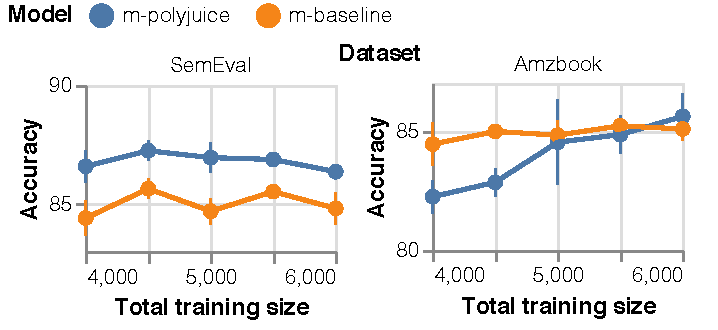
\includegraphics[width=1\columnwidth]{figures/sst_trend_2}
\vspace{-15pt}
\caption{The accuracy trend on \sst datasets, as the total training datasize $m+n$ varies. The blue line shows $m=2k$ \maug, and the orange one represents the corresponding \mcomp.
Though the counterfactuals remain useful on most datasets, too many counterfactuals may be harmful (\eg Amzbook when $m=n=2k$).
%\wts{Maybe cut/appendix?}
% (when $m+n=4k$, we have $m=n=2k$ on the orange line)
}
\vspace{-10pt}
\label{fig:sst_trend}
\end{figure}
\end{comment}


\definecolor{cfwone}{HTML}{eef5fa}
\definecolor{cfwtwo}{HTML}{daeaf5}
\definecolor{cfwthree}{HTML}{b2d2e9}
\definecolor{cfwfour}{HTML}{8abbde}

\newcommand{\fwone}[1]{\colbox{cfwone}{#1}\xspace}
\newcommand{\fwtwo}[1]{\colbox{cfwtwo}{#1}\xspace}
\newcommand{\fwthree}[1]{\colbox{cfwthree}{#1}\xspace}
\newcommand{\fwfour}[1]{\colbox{cfwfour}{#1}\xspace}

\newcommand{\fexp}[2]{\texttt{[{\color{darkgray}{#1:#2}}]}\xspace}
\newcommand{\fexptag}[1]{\fexp{TAG}{#1}}
\newcommand{\fexpfrom}[1]{\fexp{FROM}{#1}}
\newcommand{\fexpto}[1]{\fexp{TO}{#1}}
\newcommand{\fexptemp}[1]{\fexp{TEMP}{#1}}


\section{Perturbation Explanations}

%Both counterfactual explanations and semi-counterfactual explanations.
%As defined in \cite{}

\subsection{Local explanations: turning points}

\paragraph{Selection by abnormality.}
The cognitive burden of complete explanations is too great.
As a result, \citet{miller} concluded that people usually \emph{select} a small subset of (counterfactual) explanations on contrastive cases (``foils'') that they find unexpected. 
He further proposed that, as such, ``abnormality could be used to infer likely foils.''
Here, we operationalize the concept of abnormality based on \emph{the discrepancy between the expected and the actual changes in the prediction}, and use it as our selection method.

Given a prediction model $f$, we define the actual change in prediction as $d_f(\xp, x)$, and the expected prediction change as $\hat{d}_f(\xp, x)$.
The distance between the expectation and reality then becomes:
$$\Delta d_f(\xp, x) = |\hat{d}_f(\xp, x)-d_f(\xp, x)|$$
We select two abnormal, ``turning point'' counterfactuals, \ie unexpected large changes in prediction when small (large) change is expected:
$$ \xp_l = \argmax_{\xp} \Delta d_f(\xp, x), \xp_s = \argmin_{\xp} \Delta d_f(\xp, x)$$
Whereas actual prediction change is always $d_f(\xp, x)=|f(\xp)-f(x)|$ where $f(x)$ denotes the prediction probability of $f$ on $x$, $d_f(\xp, x)$ can take various forms. 
For example, as a standalone explanation method, $\hat{d}_f$ can be the cosine distance in the \emph{Embedding space}.
The embedding can be either model-agnostic (\eg with~sentence transformers~\cite{reimers-2019-sentence-bert}), or the last layer of the hidden state of the finetuned predictor.

On the other hand, as a \emph{Compensation} to existing feature attribution methods, $\hat{d}_f$ can be the importance (weights) of the perturbed tokens in $x$, estimated by feature attribution methods.
As mentioned in \wts{\S\ref{}}, methods like SHAP~\cite{} or LIME~\cite{} only estimate feature weights by \emph{masking} the words, which do not represent how model would react in non-deletion counterfactuals (replacing words or inserting negations).
Therefore, abnormalities selected in this way can  compensate or criticize the missed information, and therefore better calibrate users' trust on the predictor.


For example, consider the following \dnli instance. 
The RoBERTa model finetuned on NLI (the same as in \S\ref{subsec:contrast_set}) predicts it correctly.

\ebox{
\textbf{Premise}: The quarterback of the football team is about to be tackled by a member of the Wisconsin defensive team.\\
\textbf{Hypothesis}: The \fwtwo{quarterback} is about to be \fwone{tackled} \fwtwo{by} the \fwthree{opposing team}.\\
%\textbf{Label}: entailment\\
\textbf{Prediction} $f(x)$: entailment}

\emph{Large-invariance} $\xp_l$ then compensate SHAP by noting that changing important features do not necessarily affect the model.
Even if we change three important tokens as below, \ie, ``quarterback,'' ``opposing'' and ``team,'' the predict remains intact. 
This contrasting example suggests that the model may not handle the subjects and objects of verbs appropriately.

\ebox{
\textbf{Hypothesis}: The \swap{quarterback}{opposing team} is about to be tackled \remove{by the opposing team}.\\
\textbf{Prediction} $f(\xp)$: entailment}

Meanwhile, \emph{small-variance} $\xp_s$ notes that changing seemingly unimportant features may still change the prediction.
Though ``tackled'' is not highlighted by SHAP, some replacements (\eg ``thrown'') does affect the model:

\ebox{
\textbf{Hypothesis}: The quarterback is about to be \swap{tackled}{thrown} by the opposing team.\\
\textbf{Prediction} $f(\xp)$: contradiction}

Formally, if we denote the SHAP feature weight of a token $t$ as $w(t)$, the distance function is $d(x, \xp) = \sum_{t \in r(\xp)} w(t)$.

These surprises act as \emph{critics} to the original SHAP.
They reveal abnormality of the \emph{explainer}, but not necessarily the abnormality of the model.
In the example above, we may suspect the model to miss verbs if we merely rely on SHAP explanations. However, the small-variance shows otherwise --- the low importance results from SHAP only \emph{masking/deleting} the said verb.


\subsection{Evaluate local explanations?}
We conduct a user study to verify whether our selected counterfactual explanations help people identify model's problematic behavior.

We recruited N graduate students who have experience using model explanations before, and tasked them with a two phase experiment, where they assess the correctness of a \qqp model.
To begin, participants were given 20 \qqp examples from the validation set with labels and model predictions, but no explanations.
They were asked to assess whether they think the model would behave reasonably on variations of the example and, if not, create one perturbation where they think the model would predict incorrectly.
Then, in the second phase, they repeat the tasks as before, this time with explanations.
We evaluate on two dimensions:

%\noindent
\textbf{Q1}: 
Can the explanation effectively indicate model's abnormal behaviors around an example? 
We measured it by the number of times participants' assessment change after seeing the explanation (\eg from model reasonable to model unreasonable).

%\noindent
\textbf{Q2}: 
When they believe the model is incorrect, can the participants create perturbations that reveal the incorrectness, and is it more effective than our generated ones?
We ran the models on the collections, and count the times that the model were indeed incorrect.

\wts{The whole user study is still TODO; baseline and results; See the comment for examples generated by BERT.}


\begin{comment}
****
The examples generated by BERT.
****

  P: The quarterback of the UTEP football team is about to be tackled by a member of the Wisconsin defensive team.
  H: The quarterback is about to be tackled by the opposing team.
 Pr: entailment
 NP: Another quarterback is about to be tackled by the opposing team.
NPr: neutral
weight:  0.122
flip_unimportant_feature 0.013 {The}

  P: The quarterback of the UTEP football team is about to be tackled by a member of the Wisconsin defensive team.
  H: The quarterback is about to be tackled by the opposing team.
 Pr: entailment
 NP: Jack is about to be tackled by the opposing team.
NPr: neutral
weight:  0.461
flip_unimportant_feature 0.028 {The, quarterback}


  P: The quarterback of the UTEP football team is about to be tackled by a member of the Wisconsin defensive team.
  H: The quarterback is about to be tackled by the opposing team.
 Pr: entailment
 NP: The quarterback is about to be tackled by someone
NPr: entailment
weight:  0.218
unflip_important_feature 0.3 {team, the, ., opposing}

  P: The quarterback of the UTEP football team is about to be tackled by a member of the Wisconsin defensive team.
  H: The quarterback is about to be tackled by the opposing team.
 Pr: entailment
 NP: The quarterback is about to be tackled by the second team.
NPr: entailment
weight:  0.292
unflip_important_feature 0.149 {opposing}


\end{comment}


\subsection{Global / Interactive Explanations}
\label{subsec:global_exp}
Here, we explore more extensive use of perturbation explanations via examples, but defer more sophisticated designs and evalautions to future work.

\paragraph{Global explanations: impacts of same changes.}
Going beyond turning points for each individual data points, we can find perturbation patterns that systematically affect (preserve) model predictions.
Similar to challenge sets, the grouped perturbations then become useful for revealing model's capabilities on specific linguistic patterns.

To enable the grouping, we first featurize each perturbation $\xp$ with respect to its original instance $x$, using 
(1) its \tagstr (\fexptag{negation} for the example in Figure~\ref{fig:blank}), 
(2) its remove phrases \fexpfrom{kids}, 
(3) its added phrases \fexpto{not}, \fexpto{children}, and 
(4) the combined template \fexptemp{\swap{kids}{children}}.
For tokens involving multiple changes, we featurize both the primary and the combined changes, and so the example in Figure~\ref{fig:blank} also have additional features like \texttt{\fexptag{negation} \& \fexptag{lexical}}.

For each feature $h$ we compute the its prediction change rate over all the perturbations $\xp \in \xset_{h}$ that have the said feature: 
$R_h = \sum {\mathbb{1}[f(x) \not\eq f(\xp)]} / |\xset_h|$.

Filters on the change rate then reveal different model prediction patterns.\footnote{Because different \nli labels follow very flip patterns, we only include $f(x)=entailment$ examples here}

\noindent\textbf{Mastered patterns.}
Patterns with very high or low change rates (\eg $|R_h-0.5| > \gamma=0.3$) reveal patterns that the model has firmly learned.
In \nli, it includes \fexptemp{\swap{men}{women}} ($R_h=97\%$), \fexptemp{\swap{outdoor}{outside}} ($R_h=0\%$).

\noindent\textbf{Outliers.}
Inspecting the abnormal cases in \emph{mastered patterns}, we find harder to notice examples.
\fexptemp{\swap{three}{four}} changes the 80\% prediction(on 56 changed examples), but all the cases with affected predictions have the explicit pattern ``three'' in the premise, whereas the prediction intact ones show that the model has a hard time processing the actual counting.

\ebox{
\textbf{P}: Three girls fell on top of one another and are laughing.\\
\textbf{H}: \swap{Three}{Four} girls falling and laughing.\\
\textbf{Pr}: \swap{entailment}{contradiction}\\

\textbf{P}: Two little girls and one little boy are running.\\
\textbf{H}: \swap{Three}{Four} kids are running. \\
\textbf{Pr}: \swap{entailment}{entailment}
}

\noindent\textbf{Missed patterns.}
In contrast of the mastered cases, patterns with mild change rates (\eg $|R_h-0.5| < \gamma=0.2$) reveal patterns that the model handles unstably.
For example, the model does not handle the shuffled phrases, echoing the results from \citet{mccoy2019right}.

\ebox{
\fexptag{shuffle}, $R=0.63$ (164 cases)\\
\textbf{P}: The bride in the white dress is surrounded by the groomsmen and bridesmaids, all in black.\\
\textbf{H}: \add{white} woman \remove{in white} is surrounded by others.\\
\textbf{Pr}: \swap{entailment}{entailment}\\

%\textbf{Premise}: Man juggling apples while sitting on a couch with another man on one side and a woman on the other.\\
%\textbf{Hypothesis}: Two \swap{men}{women} sitting near a \swap{woman}{man}.
%\textbf{Prediction}: \swap{entailment}{entailment}\\

\textbf{P}: A man in a wheelchair is being pushed towards a monk.\\
\textbf{H}: The \swap{person is disabled and}{holy person} is being moved towards a \swap{holy}{disabled} person. \\
\textbf{Pr}: \swap{entailment}{entailment}
}


\paragraph{Interactive explanation.}
Besides pre-selected \emph{surprise} cases, perturbations can also support interactive explanation (ideally in a visual interface), and multi-step drill downs.
In the example: 

\ebox{
\textbf{P}: Some dogs are running on a deserted beach.\\
\textbf{H}: There is only one dog at the beach.\\
\textbf{Pr}: contradiction
}

To understand whether the model responses to quantifiers, an analyst can \BLANK ``only one'', which would reveal that the model predicts entailment correct for both perturbed hypotheses:

\ebox{
\textbf{H}: There \swap{is only one dog}{are multiple dogs} at the beach.\\
\textbf{H}: There is \swap{only}{more than} one dog at the beach.
}

Then, the analyst can keep ``more than one dog'' to inspect how the model react to other changes. 
With the model maintaining entailment on the following examples, the analyst would conclude that there may be a strong correlation between NNS and ``more than one,'' that it overwrites many of the prep constraints.

\ebox{
\textbf{H}: There is \emph{more than} one dog at the beach \add{lying down}.\\
\textbf{H}: There is \emph{more than} one dog at the beach \add{inside a cup}.\\
\textbf{H}: There is \emph{more than} one dog at the beach \add{standing}.
}


\section{Application 3: Systematic Analysis}
\label{sec:app_err_analysis}


\begin{figure}[t]
\centering
\includegraphics[trim={0 12.5cm 33cm 0cm},clip,width=1\columnwidth]{figures/err_analysis.pdf}
\vspace{-15pt}
\caption{
(A) A \nli case with a \emph{Neutral} prediction (the \uline{underlined} $f(\xp)$ are correct).
Through strict \tagstrs and blanks, \sysname generates two $\xp$ that negate the hypothesis sentence \emph{H}, which result in different predictions.
(B) Generalizing perturbation patterns beyond individual counterfactuals, we can systematically compare a model's response to different negations, \eg the prediction flips from \emph{N}eutral~$\veryshortarrow$~\emph{C}ontradiction for 92.8\% times on \swap{\texttt{DET}}{no}.
%(C) Another blank placement that leads to analyses on \emph{quantifiers}.
}
\vspace{-10pt}
\label{fig:err_analysis}
\end{figure}


Previous applications focus on a selected subset of $\xp$, but the access to the entire pool is also important.
Through a case study on the \nli RoBERTa model in \S\ref{subsec:contrast_set}, we demonstrate that \sysname's ability to generate \emph{multiple} counterfactuals per $x$ is essential for systematic error analysis~\cite{wu2019errudite}.
Here, the generation is largely driven by human analysts, and the relationship $\relation{\xp}$ can be determined by human domain expertise.


\emph{Form model behavior hypotheses by inspecting counterfactuals around one instance.}
\citet{gururangan2018annotation} asserted that negation is correlated with the class label \emph{contradiction}. 
To verify it, we can randomly select a \emph{neutral} instance $x$ as in Figure~\ref{fig:err_analysis}A, and inspect its counterfactuals that \emph{only} negate the hypothesis sentence.
\sysname produces two $\xp$:
While \exinline{is\add{n't}} seems to confirm the overfit to negation, \exinline{is not} shows a counterexample. 
We therefore hypothesize that
\emph{the model has more nuanced responses to different kinds of negations}.%, overfitting to some patterns more than others.

\emph{Verify the hypothesis through systematic counterfactual analysis.}
Does the observation generalize beyond one instance? 
We compare different negation patterns on \emph{a group of} 895 $x$ that have \emph{neutral} groundtruths and predictions.
For each $x$, we collect multiple counterfactuals by adding \ctrltag{negation} to the hypothesis, and extract \emph{negation templates} from each $\xp$ by abstracting the modified spans into linguistic features (as in Figure~\ref{fig:err_analysis}B).
Then, we select representative templates that cover various counterfactuals, and are as concrete as possible. 
The method is similar to \citet{wu2020tempura}, and more details are in Appendix~\ref{appendix:err_analysis_template}.
The top three templates selected (in bold) show interesting contrasts:
First, counter to Figure~\ref{fig:err_analysis}A, the model is relatively stable on \add{not} and \add{n't} --- they both flip around 43\% \emph{neutral} predictions to \emph{contradiction}, while maintaining others.
However, the model does respond much more aggressively to \swap{\texttt{DET}}{no}, partially confirming our hypothesis.

\begin{figure}[t]
\centering
\includegraphics[trim={0.5cm 1.8cm 32.5cm 25.5cm},clip,width=1\columnwidth]{figures/err_analysis.pdf}
\vspace{-15pt}
\caption{
Another blank placement of $x$ in Figure~\ref{fig:err_analysis}A. 
Similar changes result in different predictions (should all be \uline{\emph{Neutral}}), which leads to analyses on \emph{quantifiers}.
}
\vspace{-10pt}
\label{fig:err_analysis_quantifier}
\end{figure}


\emph{Drill-down through interactive blanking.}
If \add{not} and \add{n't} are generally stable, what causes the difference in Figure~\ref{fig:err_analysis}A?
We can drill down by adding blanks to the negated hypotheses.
For example, inspired by the returns from \exinline{\texttt{[BLANK]} is\add{n't}/\add{not} looking out the window}, we find changing \remove{woman} to \add{girl}, \add{boy}, and \add{man} in both the \emph{P} and the \emph{H} would all eliminate the \add{n't}/\add{not} difference, whereas \add{person} cannot.
Intrigued by the impact of subjects, we also apply a similar blanking to the original \emph{H}.
%: \exinline{\texttt{[BLANK]} looking out the window.}
%When the fillin is \add{two women are}, the prediction is neutral, but it flips to contradiction when the number is \add{ten}.
%When we instead use the fill in \add{more than one person is}, the model instead returns entailment.
The wild predictions in Figure~\ref{fig:err_analysis_quantifier} lead us to further hypothesize that the model does not understand quantifiers, which we verify in Appendix~\ref{appendix:err_analysis_quantifier_case}.


\paragraph{Takeaways.}
The case highlights \sysname's unique support on interactive and targeted generation.
First, the \emph{over-} generation helps analysts contrast similar perturbations, and form hypotheses that can be missed otherwise.
Human analysts rarely check both \swap{is}{is not} and \swap{is}{isn't}, and therefore can hardly realize their potential differences --- echoing our observation in \S\ref{subsec:exp_user_study} that manual counterfactual analysis may be incomplete and misleading.
Moreover, driven by the \tagstrs, \sysname allows inspecting patterns that are hard to retrieve from existing masked language models.
When applying RoBERTa to the same blanked (masked) hypotheses, we obtain less than 5\% negation counterfactuals compared to the \sysname.
Instead, more than 1,000 counterfactuals are on \swap{is}{\texttt{VERB}} and \swap{are}{\texttt{VERB}}.
Similarly, RoBERTa would not be able to produce examples in Figure~\ref{fig:err_analysis_quantifier}, as it focuses on single word replacement.
%The apparent gap highlights \sysname's support on interactive and targeted generation.

%Moreover, with \sysname diversifying the text chunks to change, it \sysname helps contrast similar changes that happen at different places.
%While \sysname enables the comparison between \swap{\texttt{VERB}}{\texttt{not VERB}} and \swap{\texttt{DET}}{no}, RoBERTa focus on changing \texttt{VERB}: the top two templates from it are \texttt{\swap{is}{VERB}} and \texttt{\swap{are}{VERB}}, producing 1000 conterfactuals in total.

\section{Related Work}
\label{sec:relate}

Counterfactuals in various applications differ by their impact on the groundtruth and model prediction labels.
Those changing the groundtruth are mostly used for counterfactual training~\cite{kaushik2019learning, teney2020learning} and evaluation~\cite{gardner2020contrast, checklist:acl20}.
As mentioned in \S\ref{sec:intro}, these counterfactuals rely heavily on human creativity and are expensive to collect.
Though it is cheaper to automate the process with parsing templates~\cite{li2020linguistically}, usually the templates are only applicable to a small subset of data.
\citet{wang2020robustness} also proposed to automatically flip the groundtruth by replacing causal word features with their antonyms.
However, they acknowledged that the method supplies limited tasks, as ``antonym'' is only well-defined in sentiment analysis.
We achieve a middle ground, and show that the team of \sysname generator and human moderator collects data more effectively.

On the other hand, multiple prior work automatically generates counterfactuals that flip the model predictions.
These methods are used for counterfactual explanations.
For example, \citet{kang2020counterfactual} guided word replacement with model prediction probabilities.
Our concurrent work, GYC~\cite{madaan2020generate} and MiCE~\cite{ross2020explaining} further enable phrase replacement through language models.
However, these methods leave out prediction-persistent explanations, which are also important as shown in \S\ref{sec:app_explain}.
If collected with additional constraints on semantic persistence~\cite{morris2020textattack, alzantot-etal-2018-generating}, the prediction-flipping counterfactuals become adversarial examples.
Despite the apparent similarities between explanations and adversarials, to the best of our knowledge, adversarial generation is still mostly through word replacement~\cite{alzantot2018generating, garg2020bae, li2020contextualized} or paraphrasing~\cite{iyyer2018adversarial, malandrakis-etal-2019-controlled}, and has yet to take advantage of language models like t5 and GPT-2 (as in MiCE and GYC).
Given the shared properties, a general-purpose model like \sysname may be more reasonable than methods tailored to specific applications.

Moreover, the emphasis on \emph{labels} greatly compresses a large set of diverse changes (\eg negations and antonym replacements both flip labels in sentiment analysis), and therefore hinders the definition and query of desired counterfactuals.
We instead design the \sysname's controls to be task (label)-agnostic and finer-grained.
Such controls additionally support application that require specifications on where and how to perturb, \eg open-ended error analysis~\cite{wu2019errudite} where contrasting similar counterfactuals is essential (\S\ref{sec:app_err_analysis}).

\begin{comment}
%%%%%%%%%%%%%%%%%%%%%%%%%%%%%%%%%%%%%%%%%%%%%%%%%%%%%%%%%%%%%%%%%%%%%%%%%%%%%%%%

\paragraph{The applications of counterfactuals.}
Counterfactuals in NLP are most broadly used for model training and evaluation.
In training, they usually augment the training data to improve model robustness~\cite{garg2019counterfactual, Wu2019ConditionalBC, Wei2019EDAED, Kumar2020DataAU} and generalizability.
\citet{kaushik2019learning} and \citet{teney2020learning} showed that counterfactual augmentations help mitigate the weights of spurious features.
%\citet{teney2020learning} further proposed to treat instances in pairs to emphasize the difference in the training process. 
%Our data can also support such experiments.
Evaluation focuses on similar aspects as training, mostly through adversarial attacks~\cite{Song2020UniversalAA}, contrast sets~\cite{kaushik2019learning} and challenge sets~\cite{Geiger2019PosingFG, liu-etal-2019-inoculation}.
We show that \sysname generated counterfactuals are also useful in such cases.

Counterfactuals also naturally support model explanations, as ``explanations are sought in response to particular counterfactual cases or foils''~\cite{miller}.
However, counterfactual explanations are much less common in NLP.
%Popular feature importance attribution methods~\cite{NIPS2017_7062, Ribeiro2016WhySI} all retrieve token importance through masking, which can be viewed as a form of (incomplete) counterfactual.
Some recent work explores this direction~\cite{ross2020explaining, vig2020causal, kang2020counterfactual}, yet the changes are usually trivial or not informative.
We seek to produce counterfactual explanations that can compensate existing explanation and analysis methods.
%Perturbation is also used for explanations, but the use is much less prominent compared to structured data.
%While counterfactual explanations have been widely advocated in structured data, the use of it in text is not yet clear. Some papers tried generation, but didn't articulate the use. %We follow the structure of X to have both counter-factual and semi-factual. 

\paragraph{Counterfactual generation.}
Existing generation methods are usually for particular applications.
Most automated ones are for adversarial examples. 
They enumerate through candidate word replacements~\cite{alzantot2018generating, garg2020bae} or paraphrases~\cite{iyyer2018adversarial, malandrakis-etal-2019-controlled} that can maintain semantic meanings while exposing model errors, but only cover limited perturbation patterns.
%The exhaustive search is hard for people to scale to~\cite{ribeiro2018sear}.
On the other hand, those evaluating and improving model decision boundaries rely on manual efforts~\cite{checklist:acl20}, which cover more diverse patterns, but at a higher cost.
Moreover, though human annotators also share strategies like negation, subject-object swapping~\cite{kaushik2019learning, gardner2020contrast}, the strategies have yet to be captured for targeted use.
Template-based methods~\cite{mccoy2019right, nie2019analyzing} are more systematic and cost-effective, but usually are only applicable to a small subset of data~\cite{li2020linguistically}.
We unify the generation for different use cases, which bridges the scalability and diversity.
We only distinguish the generated ones through posterior constraints~\cite{morris2020textattack, alzantot-etal-2018-generating}.

Some concurrent work is similar to ours, using language models to generate counterfactual sentences. 
GYC~\cite{madaan2020generate} adjusts controlled text generation methods and modifies $x$ in the latent space,  whereas MiCE~\cite{ross2020explaining} finetunes T5.
Both target at generating counterfactuals that \emph{flip the class label}, which can be useful in their use cases (GYC focusing on evaluation and MiCE aimed at explanation);
However, as there are enormous ways to flip a label, it is hard to nail down the desired perturbation from a single label signal.
We instead design the \sysname's controls to be task-agnostic and finer-grained in terms of sentence structure.
%neither approach emphasizes generality, with GYC focusing on evaluation and MiCE aimed at explanation.
%Still, they both focus on model evaluation or explanation, and therefore control the generation to \emph{flip the class label}, which may have limited scalability (\eg MiCE builds a generator for each individual task.)
%We instead finetune \sysname on general-purpose datasets, design \sysname's controls to be task-agnostic, and use them for broadening the coverage on a large variety of perturbation patterns.
Such controls additionally support application that require specifications on where and how to perturb.
\end{comment}





\section{Conclusion and Future Work}
\label{sec:discuss}

We create counterfactuals through \emph{task-agnostic} generation, and \emph{task-specific} selection.
As a result, all applications have access to the same pool of counterfactuals generated by \sysname, which are fluent, diverse, and close to the original sentence.
With additional selection methods, \sysname supports various downstream tasks, including counterfactual data augmentation, contrast set generation, counterfactual explanation, and error analysis.

One of the keys to \sysname is finetuning on paired sentences, which is the backbone for learning diverse blank placements and \tagstrs.
However, the learning inevitably comes with bias, and \sysname inherits salient contrast patterns from existing paired datasets.
For example, it is more likely to change \remove{man} to \add{woman} than \add{child}.
To further improve vocabulary diversity, we encourage the field to define more rigorous methods for finding naturally occurring sentence pairs in non-paired dataset.
We relied on heuristics of text overlap, but syntactic tree editing or knowledge graph distances may be promising.

In most of our demonstrated applications, \sysname pairs with a person, taking over the generation step and extending it beyond human rewrites or simple paraphrasing. 
As such, people can effectively focus on labeling and analyzing the counterfactuals.
We believe the human-model team is a promising framework for future work, which may involve designing control codes that better suit user needs (\eg for error analysis hypothesis testing), implementing collaborative frameworks where people and the model complement each others' generations, etc.
On the other hand, we would also like to tune the filtering and constraints, to verify that \sysname can also advance automated use cases like adversarial attacks.

We plan to open source both the \sysname model and our counterfactual selection methods.




\begin{comment}
%In tasks that require context-dependent generations --- difficult for the sentence-based model alone --- human annotators can also initiate seed counterfactuals for \sysname to extend.
%For example, to perturb question answering instances~\cite{gardner2020contrast}, the human can add the compositional reasoning steps \emph{related to} the corresponding paragraph for \sysname to perturb around.

\emph{More balanced sentence pairs and sampling.}
\sysname inherits some most most salient contrasts pairs from existing paired datasets.
For example, it is more likely to change \remove{man} to \add{woman} than \add{child}.
To further improve vocabulary diversity, we can emphasize more on \emph{finding naturally occurring sentence pairs in non-paired dataset}.
We used heuristics on text overlaps to broaden some \tagstrs, but methods like syntactic tree editing or knowledge graph distances can also be useful.



We plan to opensource both the \sysname model and the implementation of the selection methods.




\emph{Supporting existing counterfactual reasoning tools.}
Besides independent use cases, \sysname may also be plugged into existing tools that involve counterfactual generation.
%featurizing counterfactuals into Snorkel labeling functions~\cite{ratner2017snorkel} helps collect the training and evaluation data more efficiently (similar to \S\ref{subsec:global_exp}).
For example, domain experts can create perturbation tests more easily if \sysname serves as an additional building block for model testing~\cite{checklist:acl20}.
Or, they may translate $\relation{\xp}$ into labeling functions for data programming~\cite{ratner2017snorkel}.


\emph{Human-in-the-loop counterfactual generation.}
Humans can add more values than placing blanks and labeling counterfactuals, \eg supply missing perturbation patterns after seeing \sysname's generations.
In tasks that require context-dependent generations --- difficult for the sentence-based model alone --- human annotators can also initiate seed counterfactuals for \sysname to extend.
For example, to perturb question answering instances~\cite{gardner2020contrast}, the human can add the compositional reasoning steps \emph{related to} the corresponding paragraph for \sysname to perturb around.
\end{comment}

\section*{Ethical Considerations}
Our work includes labeling counterfactuals on crowdsourcing platforms, as well as conducting user studies with graduate students.
As detailed in Appendix~\ref{appendix:label_instruct} and \ref{appendix:exp_user_study}, we compensated the MTurk workers \$2.5 for ${\approx}15$ minutes of labeling, and the graduate students \$20 for the user study (one hour), above the U.S. federal minimum wage.
The studies are with IRB approval.

We only finetune GPT-2 rather than training it from scratch, such that our compute costs are relatively low (around 8 hours for finetuning, Appendix~\ref{appendix:train_data}). All of our finetuning experiments involved finetuning RoBERTa on smaller datasets.
% To reduce the cost, we may consider optimizing the finetuning dataset to reduce repetitive sentence pairs, and thereby train \sysname with fewer shots.

More critically, with most of our demonstrated applications using a human-generator hybrid mechanism, we stress that the interaction between the two deserves careful consideration.
It has long been reported that algorithms interacting with humans can negatively impact the human.\footnote{\url{https://www.nytimes.com/interactive/2017/04/02/technology/uber-drivers-psychological-tricks.html?_r=0}}
In our case, the concern might be that users can develop an over-reliance on \sysname~\cite{bansal2021does} and hastily accept its generations.
Not only can this decrease users' creativity~\cite{green-etal-2014-human}, but it may bias their analysis process: as discussed in \S\ref{sec:discuss}, \sysname generation is not exhaustive, and may favor some perturbation patterns over others in unpredictable ways.
% Hastily relying on \sysname generations may risk incomplete explorations.
In the short term, we plan to highlight these limitations as part of the model documentation, while future research should identify interaction mechanisms, so as to ensure that \sysname or other counterfactual generators support humans, rather than hindering their performance.




%\section*{Acknowledgements}
The project was supported by \tofix{ADD FUNDING INFORMATION}
We gratefully thank Scott Lundberg,Sameer Singh for their helpful comments.
We also appreciate the valuable input from our user study participants.
%Jim Chen,  Hao Peng, 
\bibliography{ref}
\bibliographystyle{acl_natbib}

\clearpage
\newpage

\appendix
%\begin{comment}
\begin{table*}[t]
\small
\centering
\setlength{\tabcolsep}{4pt}
\begin{tabular}{@{}lrrrrrrrrr@{}}
\toprule
\textbf{Dataset} & \textbf{\ctrltag{negation}} & \textbf{\ctrltag{quantifier}} & \textbf{\ctrltag{leixcal}} & \textbf{\ctrltag{resemantic}} & \textbf{\ctrltag{insert}} & \textbf{\ctrltag{delete}} & \textbf{\ctrltag{restructure}} & \textbf{\ctrltag{shuffle}} & \emph{\ctrltag{global}} \\ 
\midrule
        CAD &      3,456 &         457 &    10,650 &        4,634 &    2,169 &    2,162 &          234 &       84 &    3,756 \\
   Contrast &       336 &         436 &     1,607 &        1,291 &     589 &     586 &          275 &      149 &     877 \\
       HANS &        50 &           0 &        0 &           0 &    3,926 &    3,926 &          494 &     1,602 &       2 \\
    ParaNMT &      2,797 &         825 &    10,000 &       10000 &    6,442 &    6,205 &         5,136 &     1,417 &   10,000 \\
       PAWS &        81 &        1,815 &    10,000 &       10000 &    3,630 &    3,403 &         4,551 &    10,000 &   10,000 \\
 WinoGrande &      3,011 &          94 &    10,000 &        6,927 &     120 &     124 &          453 &       65 &    3184 \\
    \emph{Crawled} &         0 &           0 &     5,000 &           0 &    5,000 &    5,000 &            0 &      108 &    5,000 \\
      \textbf{Total} &      9,731 &        3,627 &    47,257 &       32,852 &   21,876 &   21,406 &        11,143 &    13,425 &   32,819 \\
\bottomrule
\vspace{-15pt}
\end{tabular}
\caption{The datasets used for finetuning the GPT-2 generation model, and the \tagstr distributions.}
\label{table:gpt_train_stats}
\vspace{-10pt}
\end{table*}



\section{GPT-2 as Counterfactual Generator}
\label{appendix:train_data}

\subsection{Training data collection}


We combine the following NLP datasets for finetuning \sysname.
To achieve a more balanced distribution, for each dataset, we extract \tagstrs from all the data pairs available, and randomly sample up to 10,000 instances per \tagstr.
The distribution is shown in Table~\ref{table:gpt_train_stats}.

\paragraph{Contrast set}
Authors of 10 existing NLP dataset each manually perturbed 100--1,000 instances in small but meaningful ways that change the gold label, so to inspect a model's decision boundary around a local instance~\cite{gardner2020contrast}.
The perturbation patterns vary based on the tasks and the annotators, allowing us to learn diverse strategies.
To make sure we can use the contrast set to evaluate the \sst model, we excluded the IMDb movie review from the training.\footnote{Similarly, though \qqp would be a potentially interesting dataset for training \sysname, we omitted it so \qqp can be used in our evaluation.}
%\wts{Re-train the model with other contrast sets.}


\paragraph{Counterfactually-augmented data (CAD)}
To augment the training data, \citet{kaushik2019learning} crowdsourced counterfactuals for IMDb movie review (1.7k counterfactuals on 1.7k original instances) and SNLI (6.6k counterfactuals on 1.67k original).
Similar to the contrast set, CAD's perturbation patterns vary based on the task, but can especially contribute to \ctrltag{negation}.
We split the movie review paragraphs into paired sentences, to match the sentence length of other datasets.


\paragraph{WinoGrande} is a large-scale dataset of 44k instances for testing common sense problems~\cite{sakaguchi2019winogrande}.
The dataset contains nearly identical sentences that differ only by one trigger word (\eg one noun), which flips the correct answer choice for certain questions.
The dataset is most suitable for learning lexical exchanges.

\paragraph{ParaNMT-50M} contains 50 million English-English sentential paraphrase pairs, covering various domains and styles of text, as well as different sentence structures~\cite{wieting2017paranmt}. 

\paragraph{PAWS} contains 108k paraphrasing and non-paraphrasing pairs with high lexical overlaps. 
\citet{zhang2019paws} created such challenging pairs through controlled word swapping and back translation.
As a result, the dataset demonstrates the \ctrltag{shuffle} and \ctrltag{restructure} strategies.


\paragraph{HANS} is a controlled evaluation dataset designed for testing decision boundaries of NLI models~\cite{mccoy2019right}. 
The dataset contains 10k pairs of premises and hypotheses created based on 10 heavily fallible syntactic templates, and therefore compensates rarer structural changes that may be missed by PAWS.


\paragraph{Crawled} 
We additionally crawl naturally occurring sentence pairs from non-paired datasets like SQuAD~\cite{rajpurkar-etal-2016-squad} to boost some specific patterns and increase lexical diversity. 
We estimate \emph{close} pairs using edit distance, and broadly included pairs as long as the editing is less than 60\%.
This inevitably includes cases that should not be considered counterfactuals,\eg \exinline{how do I not be} and \exinline{how do I recover it} are incorrectly considered \ctrltag{negation} pairs. 
We only include them for the most determined patterns, \ie \ctrltag{lexical}, \ctrltag{insert}, \ctrltag{delete}, and \ctrltag{shuffle}.
Among them, we further filter the pairs using \tagstrs (see the section below).
%Still, unrelated examples 


\subsection{Training Prompts \& Parameters}

Given a sentence pair, we use the two sentences interchangeably as $x$ and $\xp$ to learn the counterfactuals both ways.
For a $(x, \xp)$, we compute its primary \tagstr based on linguistic features like part-of-speech tagging or dependency trees, and blank out the changed subtrees in $\xp$.
For example, \ctrltag{negation} occurs when we observe changes on negation modifiers or specific words like ``supposedly'', and \ctrltag{shuffle} occurs when we have overlaps between tokens deleted and added.
When multiple changes occur, we label it with the primary \tagstr, which most significantly changes the semantic meaning on the corresponding subphrase.
In Figure~\ref{fig:blank}A, we use the \tagstrshort \ctrltag{negation}, as \swap{great}{not great} is more significant than \swap{kids}{children}.
If we cannot identify the \tagstr for a $(x, \xp)$ or if the editing distance is too large, we denote it with \ctrltag{global} and use it as a negative training sample.
Importantly, to allow flexible blanking at the generation time, we generate multiple training prompts from one $(x, \xp)$, with different blanking strategies: (1) just the changed tokens, (2) the associated parsing structures, (3) the merged changes, and (4) the entire sentence.
As a result, we form up to four unique training prompts given one $(x, \xp)$ pair (some examples are in Figure~\ref{fig:blank}).

%max_log_prob_diff

With the interchangeable orders and the blanks, we generate 657,144 training prompts from 191,415 sentence pairs.
We use the data to finetune an off-the-shelf GPT-2 model from \citet{Wolf2019HuggingFacesTS}, but any LM can potentially be used.
%\wts{Add the training hyperparameters; And maybe eventually move them to appendix.}
We finetuned the model for 3 epochs, with an initial learning rate 5e-5, a batch size of 16 and a sequence length of 120.


\subsection{Intrinsic Evaluations}
\label{appendix:intrinsic}






\subsubsection{Controllability with Ablation Studies}
\label{appendix:ablation_control}

We finetune another GPT-2 model with training prompts that \emph{do not} contain \tagstrs (called \emph{\sysname-a}), and quantify the impact of the \tagstrshorts through an ablation study.
For each \tagstr, we compare the \emph{control success rate} of \sysname and \sysname-a on 250 prompts (from 100 unique original sentences).
For each prompt, we generate counterfactuals through beam search (beam $=10$), and recompute the \tagstrshorts on the top three returns.
We deem the control successful if at least one of the three recomputed \tagstrshorts matches the input (though in \sysname-a, we only measure whether the \tagstrshort naturally occurs in the uncontrolled generation.)
The success rate increases by $28.4\% \pm 18.2\%$ across all \tagstrs, ranging from \ctrltag{quantifier} (increasing 8\%, from 40.4\% to 48.4\%) to \ctrltag{insert} (64.1\%, from 13.5\% to 78.6\%).
%\ctrltag{lexical} has the smallest increment \tofix{from $93\%$ to $100\%$}, mostly because \emph{\sysname-a} tend to frequently replace words.
%\ctrltag{insert} is the most impactful \tagstrshort (from \tofix{$12\%$ to $100\%$}) --- \sysname-a rarely insert additional clues on its own.

There are three common failure cases for the \tagstrshorts:
%Note that all the prompts used are guaranteed to allow the corresponding \tagstrs, and the \tagstrshorts can be less effective on more general prompts:
(1) The dual manipulation from the \tagstrs and the blanks can conflict, \eg \exinline{a dog is embraced by a \texttt{[BLANK]}} would not respond to \ctrltag{negation}.
(2) $x$ does not have a corresponding pattern. \ctrltag{shuffle} is not applicable when the sentence has only one adjective or noun (\eg \exinline{the movie is good}).
(3) Certain pattern is very prominent that it dominates the generation probability, \eg the model tends to perturb the quantifier ``two'' in \exinline{two dogs are running}, regardless of the \tagstrshort.
In the ablation study, we filtered out prompts that fell under cases 1 and 2.







\begin{table}[tb]
\small
    \centering
    %\setlength{\tabcolsep}{1.3pt}
    \begin{tabular}{lccc}
    \toprule
    \multirow{2}{*}{Model} & Diversity & \multicolumn{2}{c}{Closeness} \\
    \cmidrule(lr){2-2}
    \cmidrule(lr){3-4}
    & Self-BLEU $\uparrow$ & Semantic $\downarrow$ & Tree edit $\downarrow$ \\
    % \cmidrule{2-4}
    \midrule
    \emph{\sysname} & \textbf{0.82} & \textbf{0.37} & \textbf{2.02} \\
    Masked-LM & 0.66 & \textbf{0.27} & \textbf{1.89} \\
    PPLM-BoW & \textbf{0.82} & 0.65 & 7.65 \\
    \bottomrule
    \end{tabular}
    \vspace{-2.5mm}
    \caption{The intrinsic metrics comparing \sysname with Masked-LM and PPLM-BoW. 
    $\uparrow$ (or $\downarrow$) indicates whether the metric should be maximized (or minimized).
    As expected, \sysname counterfactuals are \emph{closer} to the original instance than PPLM-BoW, and more \emph{diverse} than the Masked-LM ones.}
    \vspace{-3mm}
    \label{table:intrinsic}
\end{table}

\subsubsection{Closeness, Diversity, Fluency}

Similar to \citet{madaan2020generate}, we verify that the \sysname generations are fluent (``plausible'' in their case) through human evaluations (\S\ref{subsec:label_efficiency}).
We also quantify the diversity and closeness by comparing it with baseline models.

For a given $x$ and its generated counterfactuals $\hat{\xset}$, we approximate \emph{diversity} using self-BLEU~\cite{malandrakis-etal-2019-controlled, zhu2018texygen} within the generated counterfactual set $\hat{\xset}$.
The higher the BLEU, the more lexically different the generated phrases are to each other (Note that this only reflects one form of $\relation{\xp}$ relationship that is task-agnostic, and is not the only possible measurement for diversity). 
Meanwhile, \emph{closeness} is measured using both the average semantic and syntactic distance between $x$ and every $\xp \in \hat{\xset}$.
We compute the semantic distance using a pretrained sentence similarity model~\cite{reimers-2019-sentence-bert}, and the syntactic one using the tree edit distance~\cite{zhang1989simple}.


We use similar baselines as \citet{madaan2020generate}: 
(1) \emph{Masked-LM}, where we blank certain parts of $x$ (by randomly placing up to three \texttt{[MASK]} tokens), and ask RoBERTa to fill in the blank.
We rely on the CheckList implementation~\cite{checklist:acl20}, as it allows filling in multiple blanks at once through beam search. 

(2) \emph{PPLM-BoW}~\cite{Dathathri2020Plug}, a model that uses bag-of-words to control the generation.
We use the first two words of $x$ as the input context (prompt), limit the length of the generation to be similar to $x$, and apply their default condition ``positive words.''
As the model generates \emph{arbitrary text} that do not depend on $x$, we agree with \citet{madaan2020generate} that PPLM-BoW should not satisfy the \emph{closeness} requirement.

We randomly select 120 instances from three classification tasks, \qqp, \nli, and \sst (40 per task), and generate 10 counterfactuals per $x$ using each of the three generators.
The averaged metrics are in Table~\ref{table:intrinsic}.
\sysname achieves compatible diversity with PPLM-BoW (self-BLEU score), and compatible \emph{closeness} with Masked-LM, achieving a balance between both.


Ideally, we would also like to compare \sysname with our concurrent work GYC~\cite{madaan2020generate} and MiCE~\cite{ross2020explaining}.
Inspired by style transfer~\cite{yang2018unsupervised} and controlled text generation, GYC performs the perturbation on the latent space of the input $x$.
Meanwhile, MiCE uses a two-step framework to generate conterfactual explanations, with the generator being T5~\cite{JMLR:v21:20-074} finetuned on the task-specific dataset.
As mentioned in \S\ref{sec:relate}, both generators focus on flipping the class label of a given $x$.
Unfortunately, both require extensive implementation or finetuning, and has yet to be opensourced.

%Still, we believe that our infilling (\texttt{BLANK}) structure will improve the \emph{closeness} over the unconstrained GYC (called content and syntactic preservation in their case).
%We also hypothesize that \sysname has better (or at least compatible) diversity than GYC. 
%Per their intended use case --- model testing and debiasing --- the control functions in GYC are driven by the predictor-of-interest (\eg sentiment classifier, NER tagger). 
%As a result, most of the GYC changes seem to focus on features deemed important by the classifier (\eg \exinline{I am very disappointed with the service} is changed by \swap{disappointed}{pleased}, \swap{disappointed}{happy}, \swap{disappointed with}{pleased to get a good}).



%

\begin{table*}[t]
\small
\centering
\setlength{\tabcolsep}{3.5pt}
\begin{tabular}{@{}l p{0.77\linewidth}@{}}
\toprule
\textbf{Application} & \textbf{Strategies} \\ 
\midrule
Data augmentation & 
    Lexical~\cite{Wu2019ConditionalBC, Wei2019EDAED, Kumar2020DataAU}\newline
    Paraphrasing~\cite{iyyer2018adversarial} \newline
    Perturbation functions~\cite{ratner2017snorkel}
\\\midrule
Counterfactual data aug. & 
    Manual~\cite{kaushik2019learning}
    Lexical~\cite{garg2019counterfactual}
\\\midrule
Adversarial attack & 
    Lexical~\cite{alzantot2018generating, garg2020bae, li-etal-2020-bert-attack, morris2020textattack, tan2020s, jin2020bert, ebrahimi2017hotflip, Zhang2019GeneratingFA, Jia2019CertifiedRT} \newline
    Template~\cite{jiang2019avoiding}\newline
    Insert~\cite{Song2020UniversalAA}
\\\midrule
Contrast set & 
    Manual~\cite{gardner2020contrast} \newline
    Templates~\cite{li2020linguistically}
\\\midrule
Challenge sets  & 
    Lexical (heuristic)~\cite{kaushik2019learning, naik2018stress} \newline
    Paraphrasing~\cite{Kavumba2019WhenCP} \newline
    Templates~\cite{Geiger2019PosingFG, kaushik2019learning, nie2019analyzing, mccoy2019right}
\\\midrule
Model analysis & 
    Lexical~\cite{garg2019counterfactual}\newline
    Template~\cite{Goodwin2020ProbingLS}\newline
    Perturbation functions~\cite{wu2019errudite, bowman-etal-2015-large, checklist:acl20}\newline
    Controlled text generation~\cite{madaan2020generate}
\\\midrule
Explanations & 
    Lexical~\cite{hase2020evaluating, vig2020causal, kang2020counterfactual} \newline
    % probably also lexical
    Lexical (through masking)~\cite{ramon2019counterfactual, ribeiro2018anchors}\newline
    Language model~\cite{ross2020explaining}
\\
\bottomrule
\end{tabular}
\vspace{-5pt}

\caption{A short survey on counterfactual application papers, and their generation strategies.}
\label{table:perturb_application}
%\end{table*}
\vspace{-10pt}

\end{table*}
%\end{comment}

\section{Survey of Perturbation Applications}
\label{appendix:paper_survey}

Table~\ref{table:perturb_application} summarizes existing applications of the counterfactuals, with their generation strategies.


\begin{figure*}
\centering
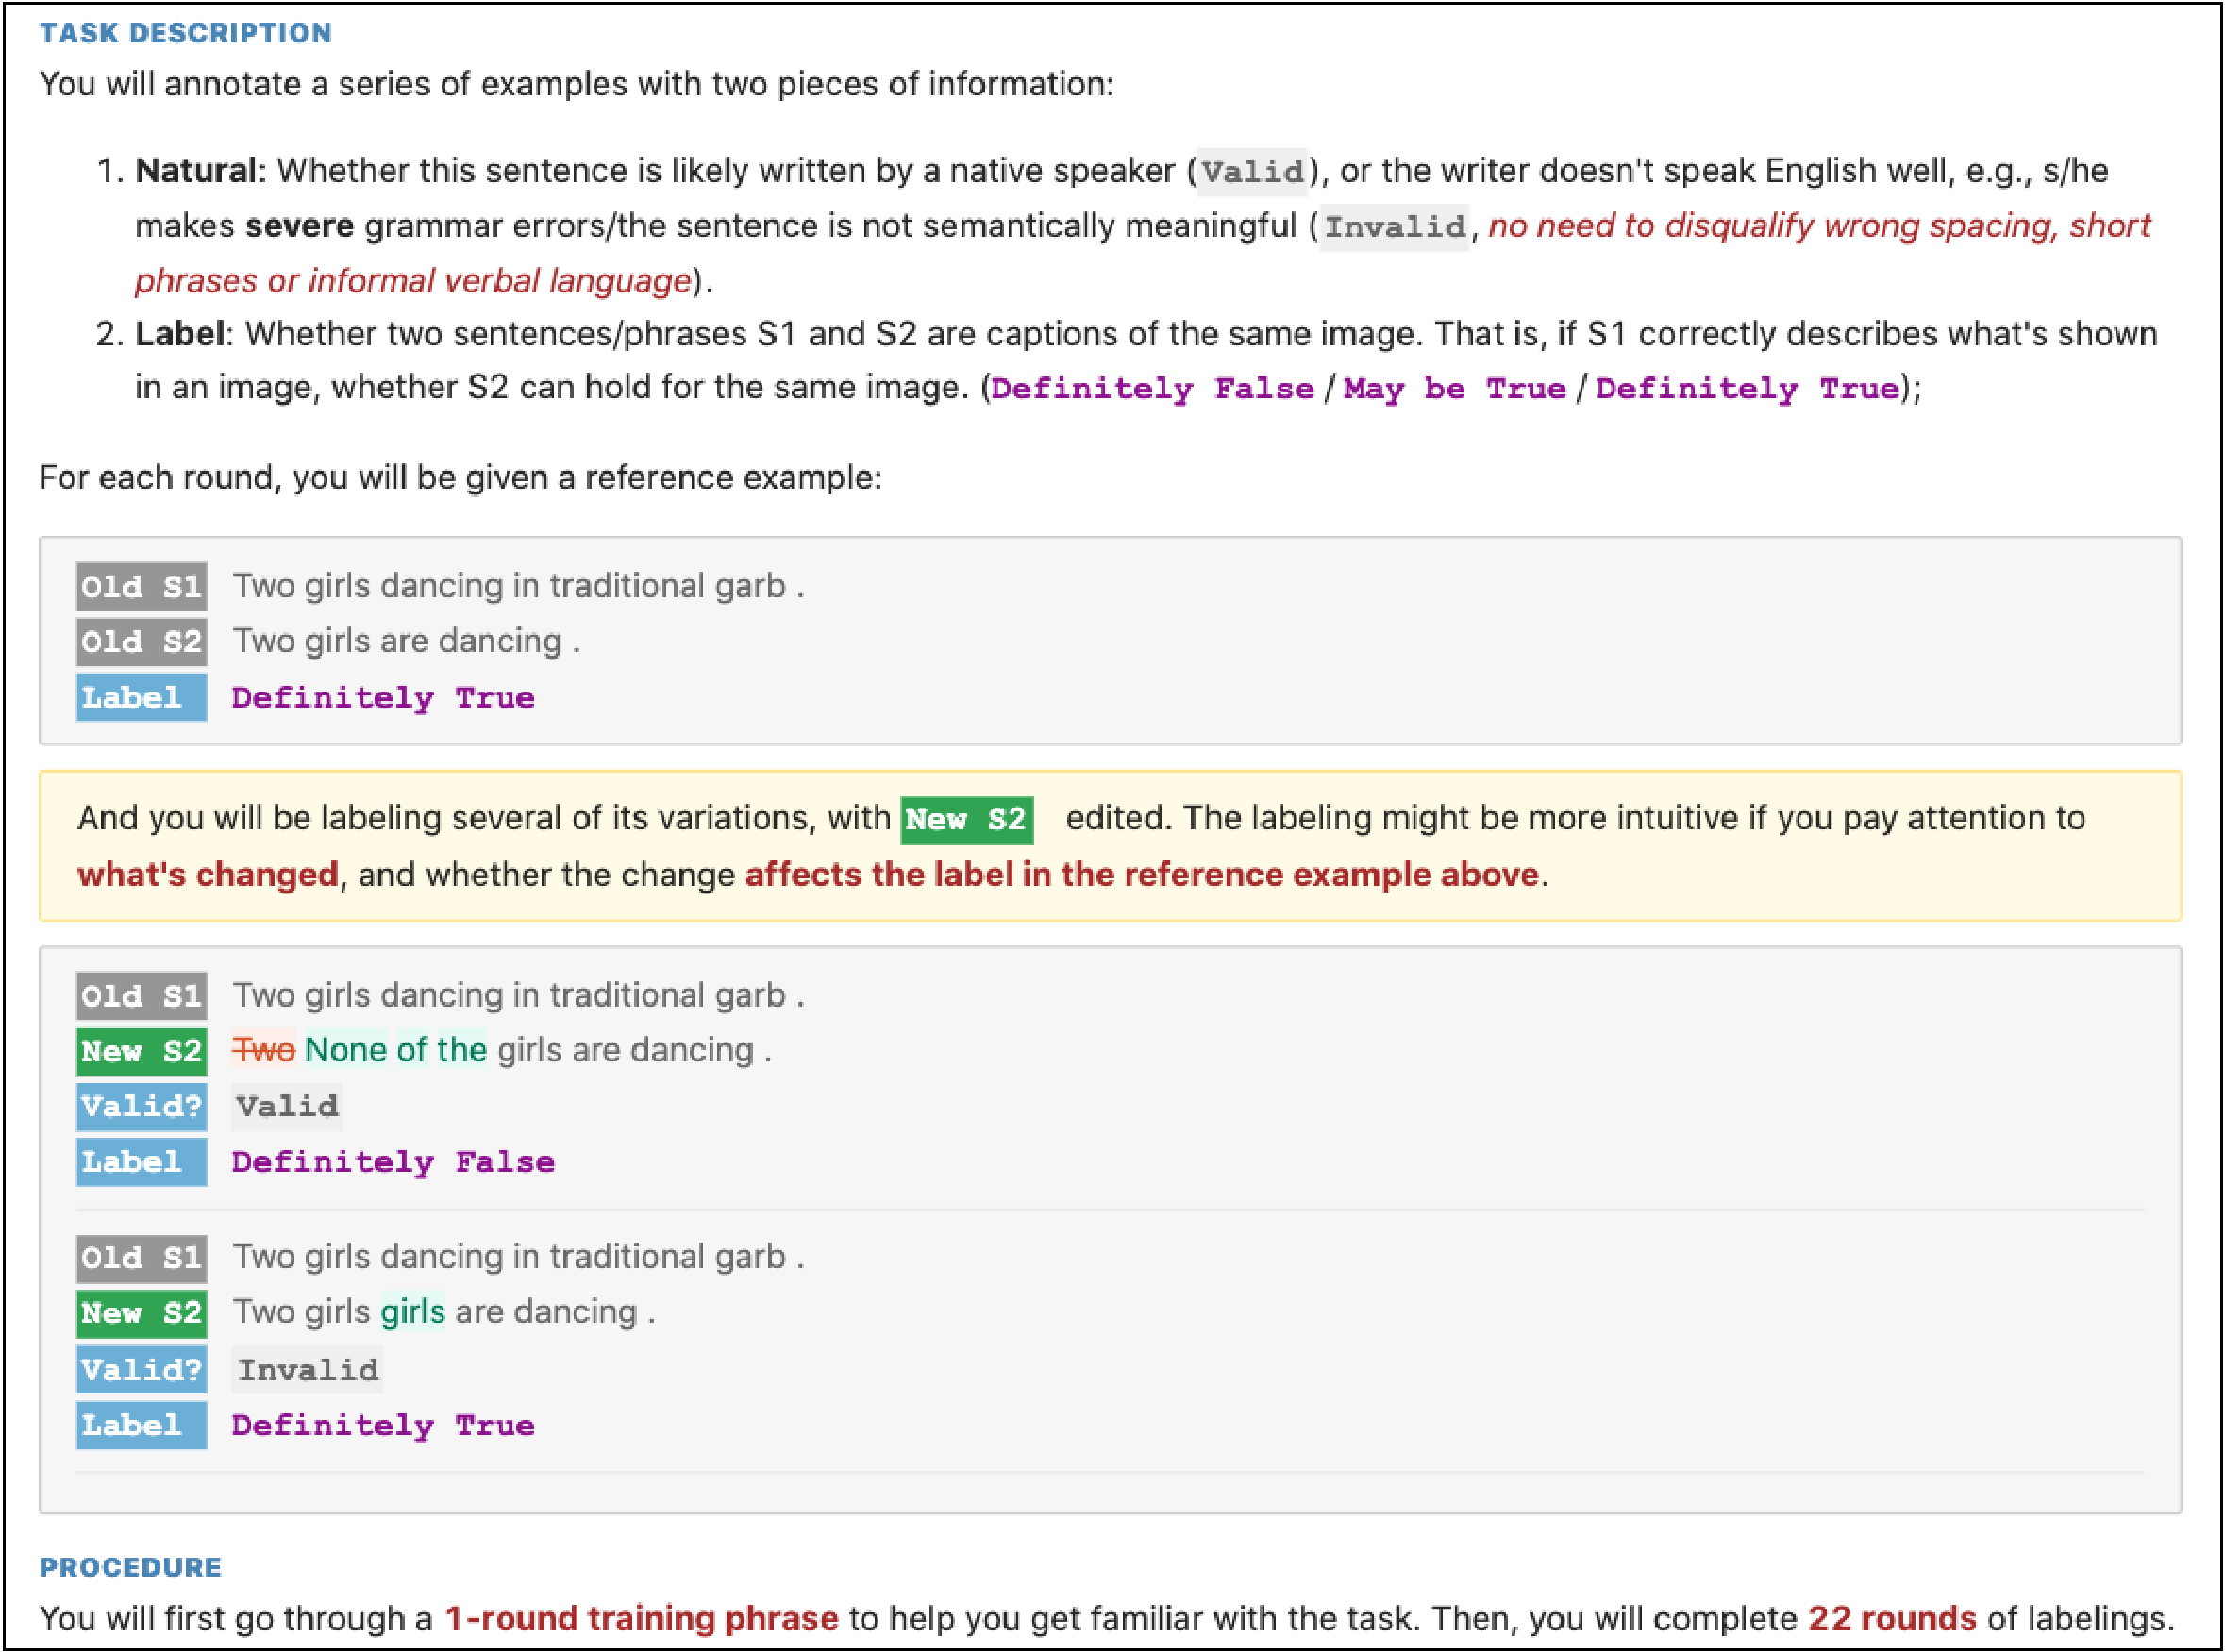
\includegraphics[width=0.9\textwidth]{figures/mturk_instruction.pdf}
\vspace{-1pt}
\caption{
The instruction for the \nli labeling task in \S\ref{sec:app_label}, with annotators labeling the perturbed hypotheses (\emph{New S2}). 
Instructions are similar for \qqp and \sst, except for the label definitions and the examples.
}
\vspace{-10pt}
\label{fig:mturk_instruction}

\end{figure*}




\section{Additional Details to Train \& Eval \S\ref{sec:app_label}}
\label{appendix:app_label}

\subsection{Tasks \& Data}
\label{appendix:app_label_data}
%We examine both evaluation and augmentation with three classification tasks: 

\textbf{Sentiment Analysis (\sst)} aims to determine the sentiment polarity of a given sentence (\emph{positive} or \emph{negative}). 
We select Stanford Sentiment Treebank (\dsst)~\cite{socher2013recursive} as the base dataset for augmentation.
It contains sentences extracted from full movie reviews on Rotten Tomatoes, which is relatively more aligned with the training data for the perturbation model. 
While the dataset also contains finer-grained labels on subphrases, we only use full sentences.
As a result, the full training data contains 6,920 sentences.

\textbf{Natural Language Inference (\nli)} is a 3-way classification task, with inputs consisting of two sentences, a premise and a hypothesis and the three possible labels being \emph{entailment}, \emph{contradiction}, and \emph{neutral}.
We augment the data based on \dnli~\cite{bowman-etal-2015-large}. 
 
\textbf{Duplicate Question Detection (\qqp)} analyzes whether two questions are duplicate of each other (i.e., if you have the answer to one question, whether you can infer the answer for the other one.) 
We use \dqqp as the base dataset~\cite{wang2018glue}, a collection of question pairs from the community question-answering website Quora.

\subsection{Diversity Ranking in \S\ref{subsec:gen_counterfactual_for_labeling}}

To select diverse counterfactuals for labeling, we first over generate a large number of candidates.
For each original example, we randomly generate up to 10 blanked sentences. Each sentence contains up to three \BLANK tokens that spread over different parsing tree structures.
We generate prompts using all the combinations of \tagstrs and blanked sentences, and collect perturbations with a beam search (for each prompt, we used 10 beams and kept top three generations.)

Then, we sample perturbations \emph{with diverse patterns} to cover more variations around local decision boundaries.
Specifically, we measure the similarity between perturbations based on weighted overlaps between their \tagstrs, the text tokens removed (denoted as $r(\xp)$) and added ($a(\xp)$), and the affected parsing tree structure $t(\xp)$. 
%For example, \ctrltag{[lexical]} \swap{man}{woman} is more similar to \ctrltag{[lexical]} \swap{man}{person} than \ctrltag{[quantifier]} \swap{man}{two men}.
%The similarity computation is in \S\ref{appendix:perturb_similarity}. 
%\wts{Need to write this part.} 
Formally, the distance between two perturbations is ($a_1$ is an abbreviation for $a(\xp_1)$):
$$d(\xp_1, \xp_2) = \alpha\cdot\mathbb{1}(s_1 = s_2) + \beta\cdot\mathbb{1}(r_1 = r_2) + \gamma\cdot\mathbb{1}(a_1=a_2)$$
With $\gamma = \beta > \alpha$ (empirically $2/5$, $2/5$, $1/5$).

\begin{figure}[h]
\centering
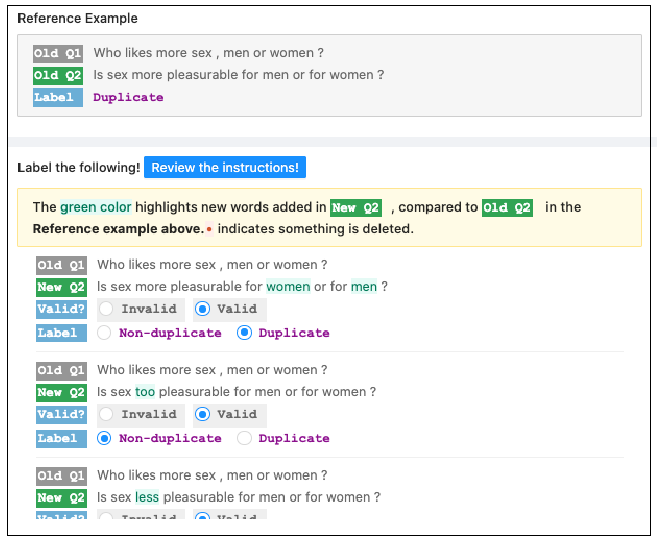
\includegraphics[width=0.9\columnwidth]{figures/mturk_label}
\vspace{-5pt}
\caption{A sample labeling task: The crowdworkers annotate three perturbations based on their validity and class label, with respect to the original instance.}
\vspace{-15pt}
\label{fig:mturk_ui}
\end{figure}




\begin{figure*}
\centering
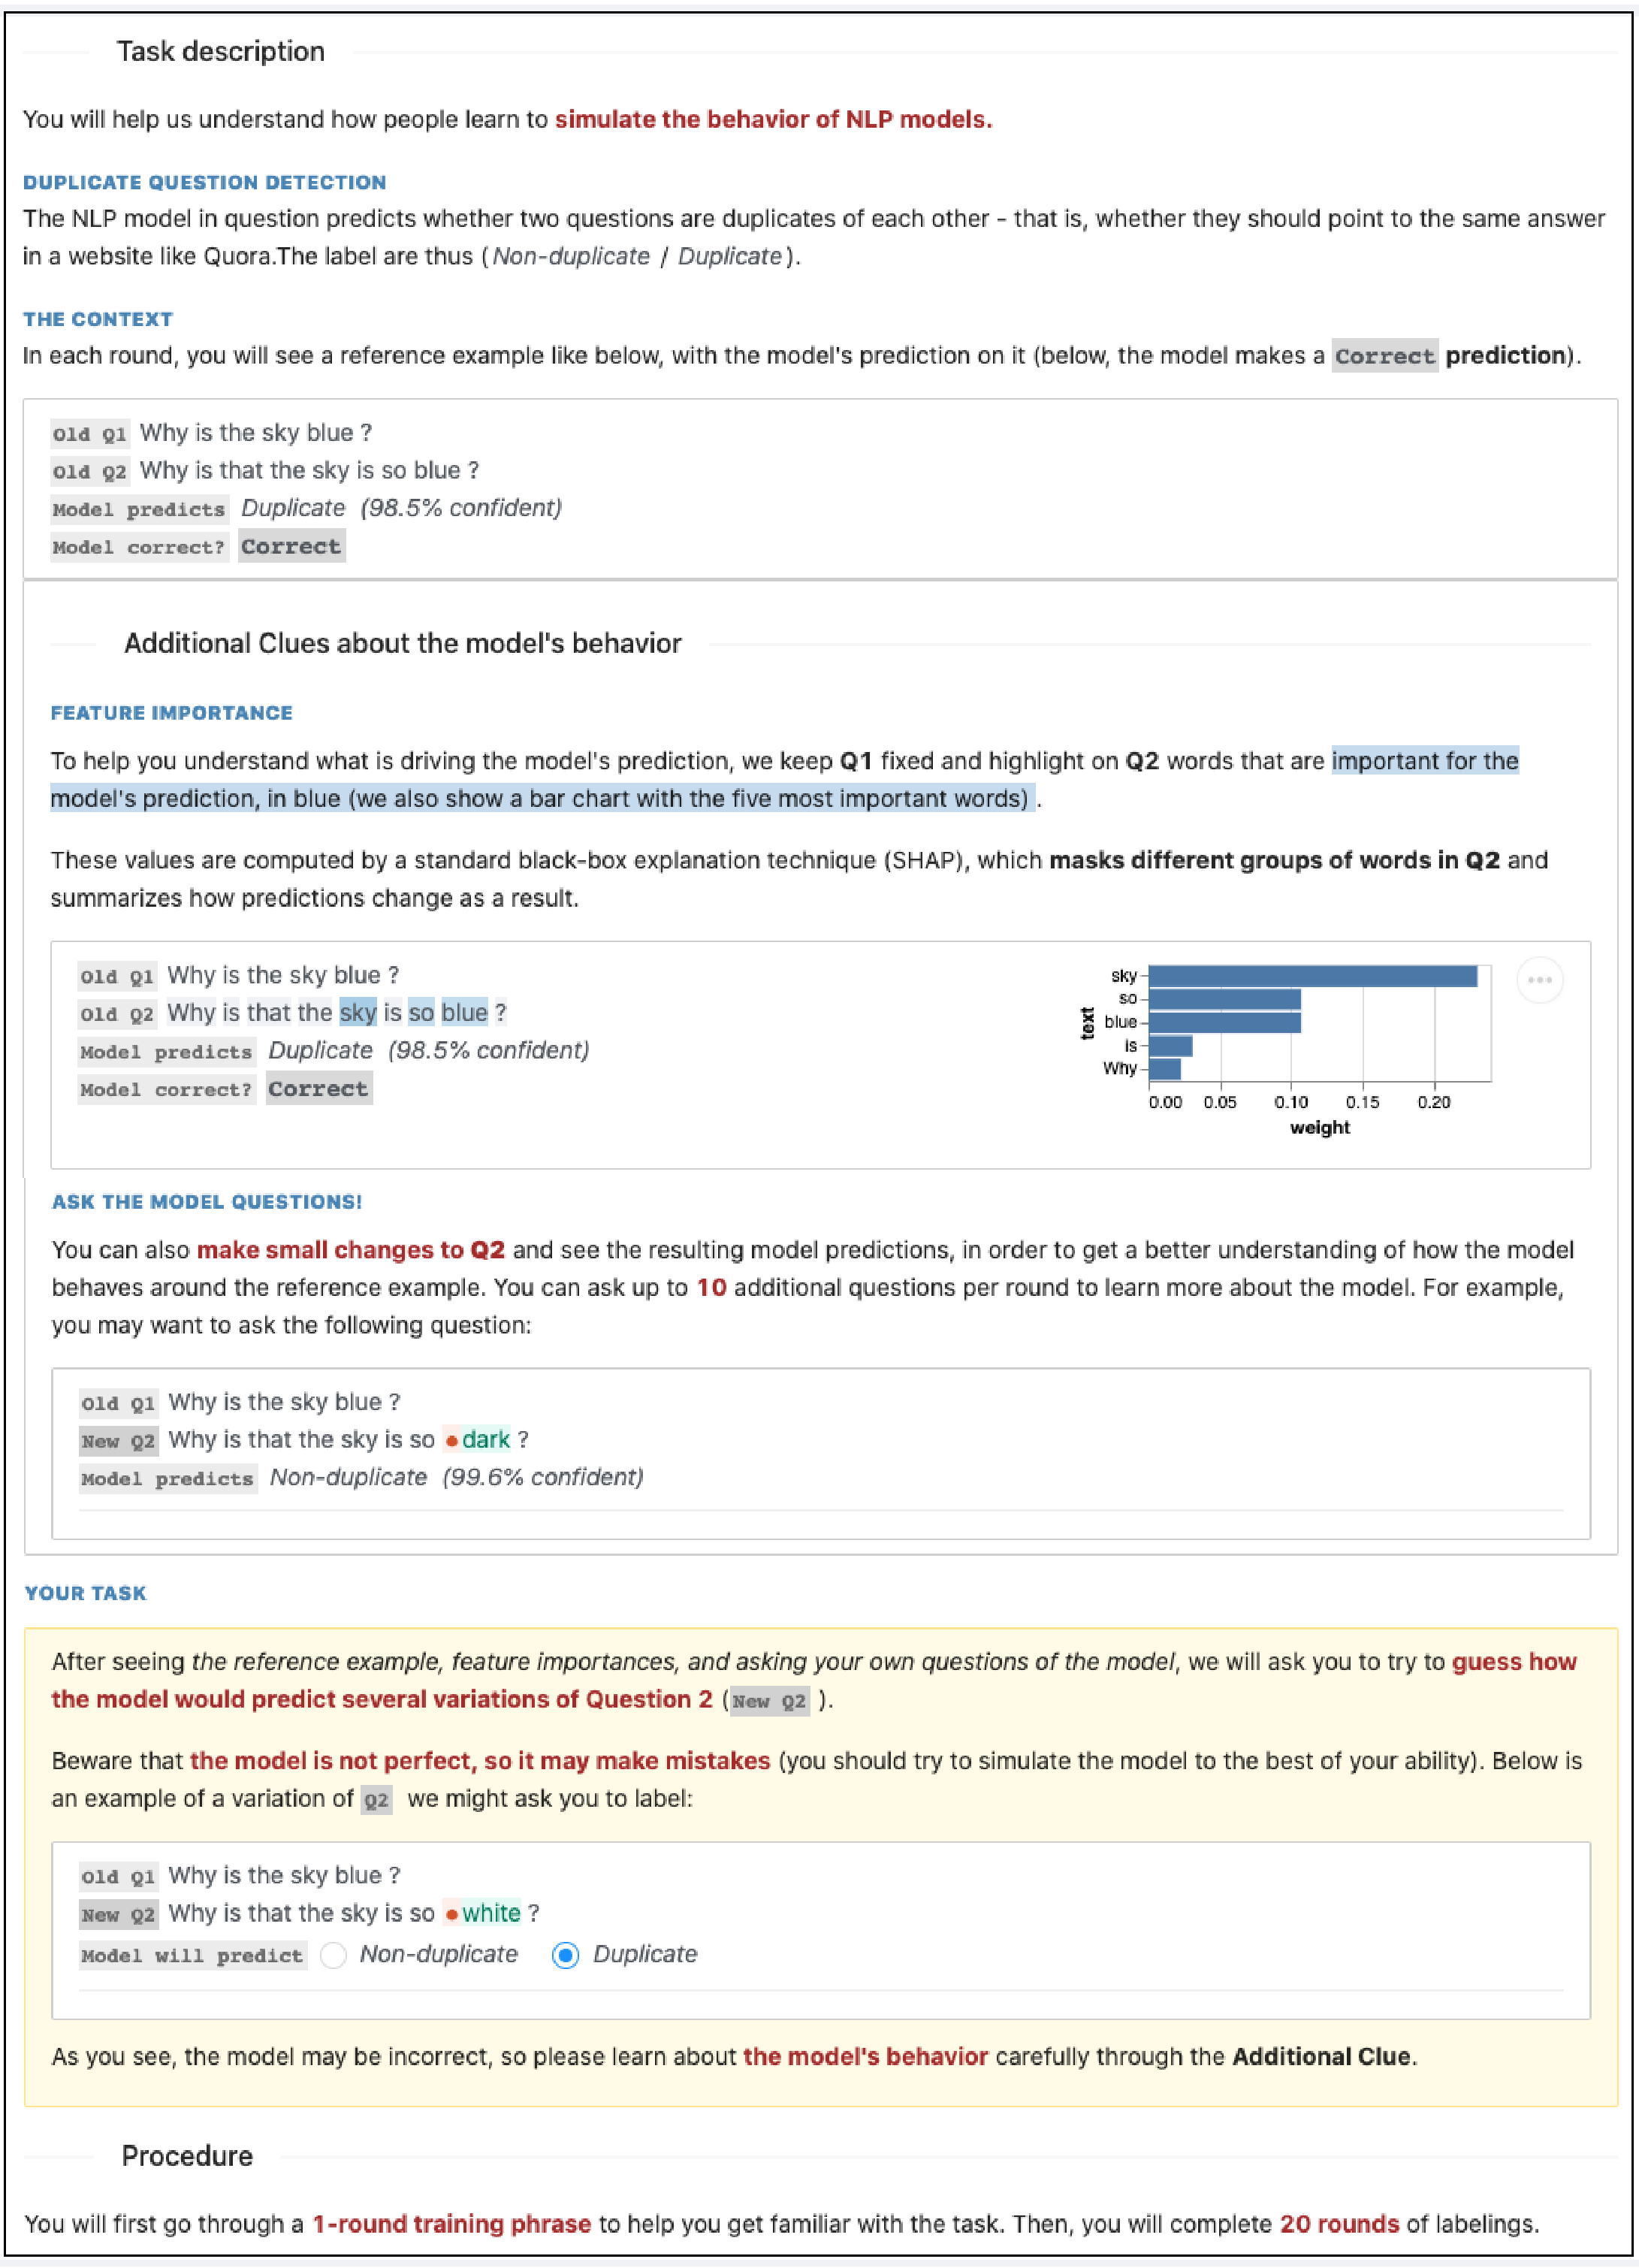
\includegraphics[width=1\textwidth]{figures/explanation_instruction}
\vspace{-15pt}
\caption{The instruction for the explanation study in \S\ref{subsec:exp_user_study}.}
\vspace{-10pt}
\label{fig:explanation_instruction}
\end{figure*}


\begin{figure*}
\centering
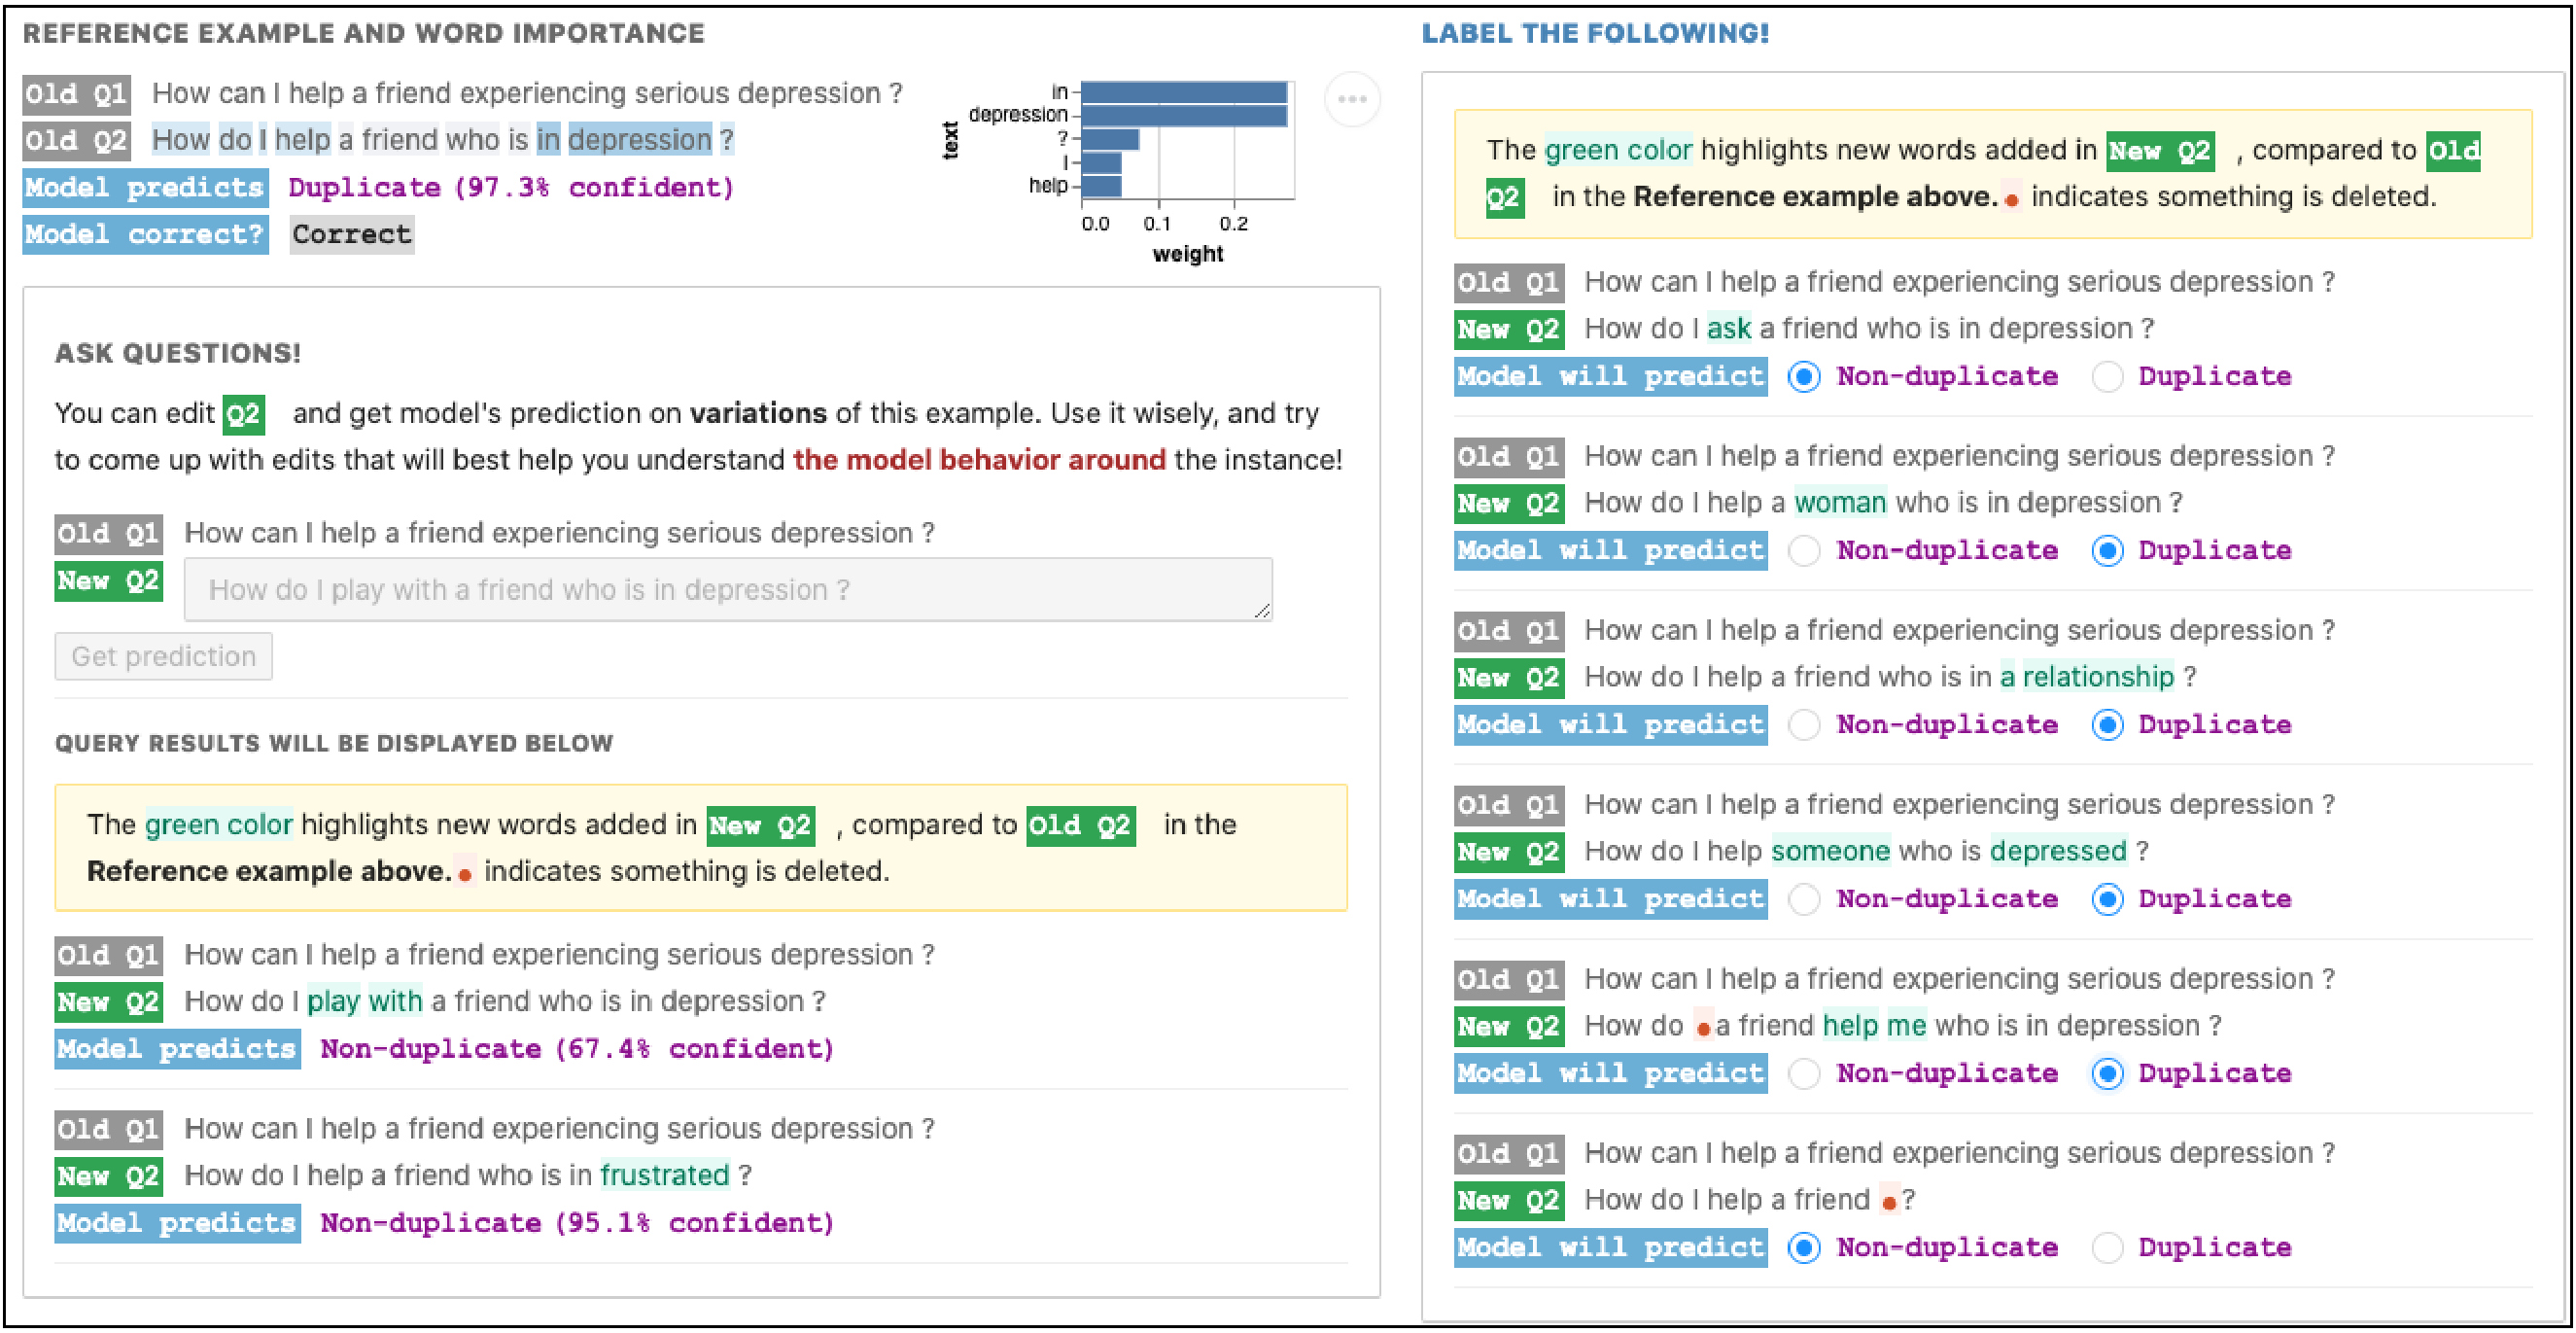
\includegraphics[width=1\textwidth]{figures/explanation_task_ui}
\vspace{-15pt}
\caption{A sample explanation interface task.}
\vspace{-10pt}
\label{fig:explanation_ui}
\end{figure*}


\subsection{MTurk Labeling Details}
\label{appendix:label_instruct}


\paragraph{Procedure}
The study started with an introduction, in which we explained the context and tasks (Figure~\ref{fig:mturk_instruction}): 
``given a reference example, the crowdworker should annotate its perturbed variations, based on whether the perturbation is valid (\emph{sounds natural}), and the classification task label.''
To familiarize them with the task, we asked them to complete 1-2 training rounds, and explained the expected labels.
The annotator then completed 22 tasks, each labeling 3 variations of a single example, as in Figure~\ref{fig:mturk_ui}.
The 22 rounds consisted of 20 actual labeling tasks and 2 extra ``gold rounds'' (6 labeled examples), with unambiguous examples and known groundtruth labels, which later served as filters for high quality crowdworkers.
As a result, each annotator contributed $20 \times 3=60$ labels.
The median task completion time was around 15-20 minutes (14.9 for \qqp, 16.7 for \sst, and 19.8 for \nli), and participants received an average payment of \$2.5 (equivalent to an hourly wage of \$7.5-10).

\paragraph{Participants}
We recruited participants from Amazon's Mechanical Turk (MTurk), limiting the pool to subjects from within the United States with a prior task approval rating of at least 97\% and a minimum of 1,000 approved tasks.

\paragraph{Data quality}
We applied two filtering strategies: 
(1) \emph{High quality worker.} 
We only kept data from participants whose median labeling time was more than 18 seconds and correctly labeled at least 4 gold examples (out of 6), or who correctly labeled all gold ones.
(2) \emph{Majority vote labeling.}
We collected two annotations per perturbation, and only kept data points that at least one annotator deems \emph{valid}, and both annotators agree on a particular \emph{class label.}

As such, when set out to collect augmentations on 1,000 original examples (thus 3,000 perturbations), we typically collect perturbations for 1,000 perturbations on 600 original examples.
One of the authors labeled a subset of 100 perturbations on 100 original examples in \sst, and reached high agreement with the majority-voted results ($\kappa=0.77$, the raw labeling agreement $88\%$).


\subsection{Training Details for \S\ref{subsec:augmentation}}
\label{appendix:data_collection}

%\paragraph{Model.}
We finetune \texttt{roberta-base} models~\cite{liu2019roberta} provided by HuggingFace Transformers~\cite{Wolf2019HuggingFacesTS}.
For each given $(m,n)$, we create three different samples of training data, and Table~\ref{table:aug_sst}--\ref{table:aug_qqp} report the average and the variance of the samples.
Each sample is further averaged over four random seeds.
For each run, we heuristically picked initial learning rates 1e-5, 2e-5, 2e-5 for \sst, \nli and \qqp, respectively, trained 20 epochs with a dropout rate of 0.1 and a batch size of 16, and selected the epoch that had the highest accuracy on the corresponding validation set (1/5 of the training data size, with the same ratio of original and perturbation examples.)
%\wts{Double check the reproducibility requirement to see if there's anything missing. And should I move the whole section to appendix?}


\section{Additional Details to Explanations \S\ref{sec:app_explain}}
\label{appendix:explanation}


\subsection{Selection Methods}
\label{appendix:exp_rank}

\paragraph{SHAP complement as local explanation}
Because the SHAP weights reflect the average effect of masking a token $t$, instead of finding just one abnormal counterfactual, we focus on \emph{word features that are abnormal on average}, \ie there is a mismatch between the importance of the changed word features and the model behavior, averaged over \emph{all counterfactuals} that have those features.

In this case, the expected change in prediction of perturbing a token $t$ is the SHAP importance on it $\E[\dist(t, x)] = s(t)$; 
For example, in Figure~\ref{fig:explanation}, $s(t=\text{``depression''})=0.276$.

The actual prediction change is the weighted average of $|\fp(x)-\fp(\xp)|$ for all the $\xp$ that affect $t$ (\swap{depression}{trouble}, \swap{depression}{a relationship}), with the weight corresponding to the number of words modified in $\xp$: If $e(\xp)$ denotes the set of edited words (replaced or deleted from $x$ in $\relation{\xp}$), then $w(\xp) = 1/|e(\xp)|$.
Intuitively, the more words changed in $\xp$, the less effect each word has; In Figure~\ref{fig:explanation}D, we regard ``depression'' to be responsible for half of the impact on changing \swap{in depression}{suicidal}.

We group the counterfactuals based on their affected words $G_t = \{\xp\ |\ t \in e(\xp)\}$. $\dist(t, x)$ then becomes:
$$\dist(t, x) = \frac{1}{|G_t|+1} \left(s(t) + \sum_{\xp \in G_t} w(t)\cdot |\fp(x)-\fp(\xp)|\right)$$
We add the additional SHAP weight $s(t)$ as a smoothing factor to punish dominating outlier $\xp$.
Then the gap between the expectation and the reality is (similar to \S\ref{subsec:local_explain}):
$$\Delta\dist(t, x) = \dist(t, x)-\E[\dist(t, x)]$$
We first find the abnormal tokens: (1) $t$ with small SHAP weight, but $\xp$ that change $t$ experience large prediction change on average: $t_L = \argmax_{t\in x} \Delta\dist(t, x)$, and (2) $t$ with large SHAP weight, but $\xp$ with $t$ changed usually have intact prediction: $t_U = \argmax_{t\in x} -\Delta\dist(t, x)$.

Then, we use the most extreme cases within the groups of $G_{t_L}$ and $G_{t_U}$ as the concrete counterfactual explanations, based on their prediction change $|\fp(x)-\fp(\xp)|$, and the aggregated SHAP weights of all the changed tokens:
$$\xp_L = \argmax_{\xp \in G_{t_L}} \left( |f_p(x)-f_p(\xp)| - \sum_{u\in r(\xp)} s(u) \right)$$ 



\paragraph{Global explanation}
To enable the grouping, we first featurize each counterfactual $\xp$ with respect to its original instance $x$, using 
(1) its \tagstr (\fexptag{negation} for the example in Figure~\ref{fig:blank}), 
(2) its remove phrases \fexpfrom{kids}, 
(3) its added phrases \fexpto{not}, \fexpto{children}, and 
(4) the combined template \fexptemp{\swap{kids}{children}}.
For tokens involving multiple changes, we featurize both the primary and the combined changes, and so the example in Figure~\ref{fig:blank} also have additional features like \texttt{\fexptag{negation} \& \fexptag{lexical}}.
These features form the relationship $\relation{\xp}$ in use.

For each feature $h \in \relation{\xp}$, we build a group of counterfactuals that contain $h$ (of course, these also include their corresponding $x$): $G_h = \{ \xp\ |\ h\in \relation{\xp} \}$.
We compute the probability of the predicted label changes all the $\xp \in G_{h}$: $Pr(y_1, y_2) = |G_h^{y_1\veryshortarrow y_2}|/|G_h|$, where $ G_h^{y_1\veryshortarrow y_2} = \{ (x, \xp)\ |\ (x, \xp) \in G_h, f(x)=y_1, f(\xp) = y_2 \}$.
The abnormality of a feature $h$ is represented by the entropy of the prediction change:
$$I_h = -\sum_{y_1 \in Y, y_2 \in Y} Pr(y_1, y_2) \cdot \log Pr(y_1, y_2)$$
We find the abormal feature with $\hat{h} = \argmin I_h$.



\subsection{User Study Details}
\label{appendix:exp_user_study}

The instruction for the user study in \S\ref{subsec:exp_user_study} is in Figure~\ref{fig:explanation_instruction}, and Figure~\ref{fig:explanation_ui} shows the sample interface for one round. 
Participants started by just seeing the reference example and the model query box on the left hand side.
When they chose to start the task or after they had exhausted their ten query chances, the query box was disabled, the tasks on the right were displayed, and the participants complete the tasks.
\section{Additional Err. Analysis Details \S\ref{sec:app_err_analysis}}
\label{appendix:err_analysis}

\subsection{Additional Case Study: Quantifiers}
\label{appendix:err_analysis_quantifier_case}

\begin{figure}[t]
\centering
\includegraphics[trim={0 25.2cm 34.5cm 0cm},clip,width=1\columnwidth]{figures/err_analysis_two_three}
\vspace{-20pt}
\caption{
The \nli model cannot perform the actual counting when the exact number is missing from \emph{P}.
%In (B), it still predicts (the now incorrect) \emph{Entailment}.
}
\vspace{-10pt}
\label{fig:err_analysis_two_three}
\end{figure}


%\citet{gururangan2018annotation} also mentioned that one common strategy for creating NLI examples is to modify the numbers, suggesting that the model should have seen various examples related to numbers.

As a follow-up to Figure~\ref{fig:err_analysis_quantifier}, we slice the data to find \emph{entailment} instances that have numbers in the hypothesis sentence, and perturb their \ctrltag{quantifiers}.
The extracted templates show that the model does not perform actual counting. 
When changing one number to another (\swap{\texttt{NUM}}{\texttt{NUM}}), the model only flips the label in 64.7\% cases, while we would expect all cases to be like in Figure~\ref{fig:err_analysis_two_three}A.
An inspection of instances indicates the model gets confused when the premise does not contain a number explicitly. 
Indeed, when we filter for such instances (e.g. Figure~\ref{fig:err_analysis_two_three}B), the label flip rate of \swap{\texttt{NUM}}{\texttt{NUM}} is lowered to 30.2\%.

Further, the model only reacts to \emph{some} quantifier phrase modifiers. 
\addplus{at least} (\exinline{\add{at least} two women are at a bar}) will always still result in \emph{entailment}, prediction, \addplus{only} and \swap{}{exactly} flip the predicted label to \emph{neutral} 90\% of the time (\exinline{\add{exactly} two women are at a bar}), but the model only changes the prediction 52.6\% of the time when we add \addplus{more than} (\exinline{\add{more than} two women are at a bar}).


\subsection{Representative Perturbation Templates}
\label{appendix:err_analysis_template}

Similar to \citet{wu2020tempura}, the process of finding representative perturbation patterns takes two steps:

\textbf{Extract template.}
For each $\xp$, we compare it with its $x$, and translate the perturbed spans into templates using different combinations of texts, lemmas, sparse and fine-grained part-of-speech tags.
We optionally include surrounding contexts determined by the parsing tree structure (tokens that share the same parents as the perturbed span).
For example, \exinline{is \add{not} reading} can result in templates $t$ as fine-grained as \swap{is reading}{is not reading}, or as sparse as \addplus{\texttt{PART}}.
Meanwhile, \exinline{are \add{not} playing} also translates to \addplus{\texttt{PART}} or \addplus{\texttt{not}}, but not \swap{is reading}{is not reading}.
As such, the $\xp$ and templates form a many-to-many relationship: each $\xp$ generates multiple templates, and each template covers a different group of $\xp$.

\textbf{Select Representative Templates.}
To find representative changes, we prefer (1) templates that cover a large number of $\xp$.
Meanwhile, to avoid overfitting to one instance (\eg extracting a template \swap{red}{\texttt{ADJ}} only because ``red'' is repeatedly perturbed in one $x$), we prefer (2) templates that perturb various unique $x$.
We also prefer (3) finer-grained templates, to avoid being unnecessarily abstract (\eg to avoid abstracting ``not'' when it is the only \texttt{PART} changed.)

%$\hat{\xset}_i$

With these intuitions, we form the template selection as a weighted set coverage problem.
We see the union of counterfactuals for each $x$, $\hat{\xset}$, as the entire set of elements.
Then, each template $t \in T = {t_1,...,t_m}$ represents a subset of $\hat{\xset}$ that contains a number of counterfactuals $|t|$.
We define the weight as $w(t) = g(t) / |t|_x$, where $|t|_x$ quantifies the unique original $x$ covered by $t$, and $g(t)$ represents the sparsity of $t$ (heuristically decreasing from \texttt{text} to \texttt{POS}).
This way, templates that are too abstract or too focused on a certain $x$ are penalized by having a high weight. 
We use a classic greedy algorithm~\cite{vazirani2013approximation} to select a subset of $T^* \subset T$, such that the aggregated coverage is maximized, and the weight is minimized.


%\balance
%
\begin{table*}[bp]
\small
\centering
\begin{tabular}{p{0.95\linewidth}}
\toprule
\textbf{Additional examples} \\ 
\midrule
It sucked \add{me in}. \\
\midrule

For those who are intrigued by politics of the '70s , the film is every bit as \swap{fascinating}{flawed} as it is \swap{flawed}{intriguing}. \\
\midrule

So exaggerated and broad that it comes off as \swap{annoying}{engaging} rather than \swap{charming}{annoying}. \\
\midrule

The film \swap{delivers}{doesn't deliver} what it promises: A look at the ``wild ride'' that ensues when brash young men set out to conquer the online world with laptops, cell phones and sketchy business plans. \\
\midrule

It's a crime movie made by someone who obviously knows \swap{nothing}{much} about crime. \\
\midrule

\swap{Even with}{Despite} all its botches, Enigma offers \swap{all}{none of} the pleasure of a handsome and well-made entertainment .\\
\midrule

``Catch Me'' feels \add{almost} capable of charming the masses with star power, a pop-induced score and sentimental moments that have become a Spielberg trademark.\\
\midrule

A sentimental but entirely \swap{irresistible}{unentertaining} portrait of three aging sisters.\\
\midrule

This is a movie full of \swap{grace}{mistakes} and, ultimately, \add{no} hope.\\
\midrule

Its simplicity puts an exclamation point on the fact that this isn't something to be taken seriously, but it also \swap{wrecks any chance}{poses an opportunity} of the movie rising above similar fare.\\
\midrule


\swap{If}{Even if} the film \swap{fails to fulfill}{succeeds in fulfilling} its own ambitious goals , it \swap{nonetheless sustains}{fails to sustain} interest during the long build-up of expository material .\\

\bottomrule
\end{tabular}
\vspace{-5pt}
\caption{Additional examples for Sentiment Analysis.}
%\wts{Change all the examples to be on an identical sentence, not all different cases. And consider further annotate the tags based on whether they just do semantic change or also syntactic change.}}
\label{table:sst_example}
\vspace{-10pt}
\end{table*}


\begin{table*}[bp]
\small
\centering
\begin{tabular}{p{0.95\linewidth}}
\toprule
\textbf{Additional examples} \\ 
\midrule


\textbf{Q1}: Poor people are more generous than rich people. Why? \newline
\textbf{Q2}: Is it true \swap{poor}{rich} people are more generous than \swap{rich}{poor} people? \\
\textbf{Q2}: Is it true poor people \swap{are more generous}{give more to charities} than rich people? \\
\midrule

\textbf{Q1}: Are TripAdvisor reviews more reliable than Yelp reviews because of their review process \newline
\textbf{Q2}: Are TripAdvisor reviews \swap{more}{less} reliable than Yelp reviews? \newline
\textbf{Q2}: Are TripAdvisor reviews more \swap{reliable}{unreliable} than Yelp reviews? \newline
\textbf{Q2}: Are \swap{TripAdvisor}{Yelp} reviews more reliable than \swap{Yelp}{TripAdvisor} reviews? \\
\midrule

\textbf{Q1}: How do you describe a smell? \newline
\textbf{Q2}: How will you describe a smell \swap{to}{from} a person? \newline
\textbf{Q2}: How will you describe a \swap{sound}{smell} to a person? \\
\midrule

\textbf{Q1}: Why are most psychopaths males and not females?and are female psychopaths different from male psychopaths? \newline
\textbf{Q2}: Is there a difference between male \remove{and female} psychopaths? \newline
\textbf{Q2}: Is there a difference between male and female \remove{psychopaths}? \newline
\textbf{Q2}: \add{Why} is there a difference between male and female psychopaths? \\
\midrule

\textbf{Q1}: How can I loose 5kgs weight in a week without exercise? \newline
\textbf{Q2}: How can I lose weight \swap{without}{by} doing exercise? \newline
\textbf{Q2}: How can I lose weight \remove{without doing exercise}? \newline
\textbf{Q2}: \swap{How can I}{Why can't you} lose weight without doing exercise? \\

\bottomrule
\end{tabular}
\vspace{-5pt}
\caption{Additional examples for Duplicate Question Detection, with the Q1 intact and Q2 changed.}
%\wts{Change all the examples to be on an identical sentence, not all different cases. And consider further annotate the tags based on whether they just do semantic change or also syntactic change.}}
\label{table:qqp_example}
\vspace{-10pt}
\end{table*}


\begin{table*}[bp]
\small
\centering
\begin{tabular}{p{0.95\linewidth}}
\toprule
\textbf{Additional examples} \\ 
\midrule

\textbf{P: }A small child stands in front of short white table.\newline
\textbf{H: }A child \swap{near}{sitting on} a table.\\
\midrule


\textbf{P: }A child sticks his head through a hole to create a picture of his head being a flower blossom\newline
\textbf{H: }The child is poking his head \swap{through}{to see} something.\\
\midrule

\textbf{P: }A young woman is playing fool.\newline
\textbf{H: }The woman is \swap{old}{very young} and not playing any games.\\
\midrule

\textbf{P: }Metal supports make a repeating X shape along the wall of the station.\newline
\textbf{H: }The walls are stronger with \swap{metal}{wood} supports rather than \swap{wood}{metal fences}.\newline
\textbf{H: }The walls are \swap{stronger}{less sturdy} with metal supports rather than wood.\\
\midrule

\textbf{P: }Several gentlemen are speaking into a microphone and the man in the glasses appears to be saying something funny\newline
\textbf{H: }Somebody \swap{that is shown wears}{shows} glasses.\\

\bottomrule
\end{tabular}
\vspace{-5pt}
\caption{Additional examples for Natural Language Inference, with the \textbf{P}remise intact and \textbf{H}ypothesis changed.}
%\wts{Change all the examples to be on an identical sentence, not all different cases. And consider further annotate the tags based on whether they just do semantic change or also syntactic change.}}
\label{table:nli_example}
\vspace{-10pt}
\end{table*}


\section{Additional counterfactuals}
Here, we include some additional counterfactual for each classification task.


\end{document}
